% Standard A4 size
\documentclass[a4paper, report]{jsbook}

% Standard A4 size with 10pt font
%\documentclass[a4paper, 10pt, report]{jsbook}

% A5 size
%\documentclass[a5paper, landscape, report]{jsbook}
%\AtBeginDocument{\special{papersize=\the\paperwidth,\the\paperheight}}
\usepackage[top=15truemm,bottom=15truemm,left=15truemm,right=15truemm]{geometry}


\usepackage[dvipdfmx]{graphicx}
%\usepackage{graphicx}

\usepackage[titletoc,toc,title]{appendix}
\usepackage{amsmath,amssymb}
\usepackage{ascmac}
\usepackage{braket}
\usepackage{makeidx}
\makeindex
\usepackage{textcomp}

\usepackage{comment}
\makeatletter
  \renewcommand{\theequation}{\thechapter.\arabic{equation}}
    \@addtoreset{equation}{chapter}
  \renewcommand{\thefigure}{\thechapter.\arabic{figure}}
    \@addtoreset{figure}{chapter}
  \renewcommand{\thefootnote}{注\thechapter.\arabic{footnote}}
    \@addtoreset{footnote}{chapter}
 \makeatother
  
\begin{document}

\title{光と物質の量子論(前半)\\}
\author{東京大学大学院工学系研究科電気系工学専攻\\小関泰之}
\frontmatter
\maketitle

%\begin{comment}
	
\begin{comment}
\chapter{修正記録}
\begin{itemize}
	\item 2017/7/7 書き始め。
	\item 2017/8/17 光増幅まで一通り書いた。
\end{itemize}
8/17 全体の構成についてのレビュー
\begin{itemize}
	\item 干渉検出、ビームスプリッタ等は1章に持ってくるべき。
	\item 量子力学のおさらいが長い。証明はAppendixに持っていく。
	\item 重要なメッセージを章の最後に書く。
\end{itemize}

2章のまとめを書いていない

疑問:ビームスプリッタのハミルトニアンの固有状態と固有値は?

その前に、変位演算子のハミルトニアンの固有状態は?$\alpha = -i$とすると、
\begin{equation}
  \hat H_d = \hbar(\hat a + \hat a^\dagger)
\end{equation}
これはエルミートなので必ず固有状態をもつ。
\begin{equation}
  \ket \psi = \delta(Q)
\end{equation}
固有値は$Q$。なので、変位演算子によって$-P$方向にシフトする。

このことを用いてバランスド検出の説明を試みる?

大事な項目を最後にまとめる。

最終的には、$\hat Q, \hat P$での表現を全て$\hat x, \hat y$に一本化したい。

位置$Q$を基底とする場合

$\hat H_c = \hbar(\hat a \hat b^\dagger + \hat a^\dagger \hat b)$の固有状態:$\ket{\phi_{1\pm}} = \frac 1 {\sqrt 2}(\ket 1 \ket 0 \pm \ket 0\ket 1) $(シングルフォトンの場合。$\ket {\phi_\pm}$は直積で書けない。これはエンタングル状態であることを示している。)

$\ket {\phi_{2\pm}} = \ket 2 \ket 0 \pm \sqrt 2\ket 1 \ket 1 + \ket 0 \ket 2$

$\hat H_c\ket{\phi_{2\pm}} = \hbar(\sqrt 2 \ket 1 \ket 1 \pm 2\ket 0 \ket 2 \pm 2\ket 2 \ket 0 + \sqrt 2 \ket 1 \ket 1) = \pm \sqrt 2\hbar \ket {\phi_{2\pm}}$ 

直積についての説明を書く。

参考文献リストを作っておく。


\textbf{行うことリスト}
\begin{itemize}
	\item 絵を描く。
\end{itemize}


\begin{table}
	
\begin{center}
	
\caption{操作の演算子とその意味}
\begin{tabular}{c c}
\hline
演算子 & 意味\\
\hline \hline
$\hat H = \hbar \omega (\hat a_1^2 + \hat a_2^2) = \hbar \omega (\hat a^\dagger \hat a + 1/2)$& 調和振動子のハミルトニアン\\
$U(t) = \exp(\hat H t/ i\hbar )$& 時間発展演算子\\
$D(\alpha) = \exp(\alpha \hat a^\dagger - \alpha^*\hat a)$& 変位演算子\\
$\hat H_d = i\hbar(\alpha \hat a^\dagger - \alpha^* \hat a)$& 変位のハミルトニアン\\
$\hat H_c = \hbar(\hat a \hat b^\dagger + \hat a^\dagger \hat b)$& 2モード結合のハミルトニアン\\
$\hat H_a = \hbar(\hat a \hat b + \hat a^\dagger \hat b^\dagger)$& 光増幅のハミルトニアン\\
\hline
\end{tabular}

\end{center}
\end{table}

\begin{table}
\begin{center}
	\caption{特殊な量子状態}
	\begin{tabular}{c c}
	\hline
		ケット & 意味\\
		\hline \hline
		$\ket n$ & 光子数$n$の光子数状態\\
		$\ket \alpha$ & 複素振幅$\alpha$のコヒーレント状態\\
		\hline
	\end{tabular}
\end{center}
\end{table}
\end{comment}

\chapter{はじめに}


光は光子(フォトン)と呼ばれる粒子の集まりである。光が粒子であるということ(量子性)は、光を用いて通信、制御、計測を行う際において雑音として現れ、性能や精度の物理限界を与える。光を用いた計測技術の高精度化・高感度化や光通信の大容量化を図るうえで、その限界を知り、限界を高めていくことは重要であり、そのためには光の量子性に関する理解も欠かせない。また、近年では光の量子性を積極的に活用することで、量子暗号、量子テレポーテーション、量子コンピューティング等の技術の開発も進められている。これらの光の量子性を扱う学問を量子光学という。

光の検出法には様々な種類があり、それは光の強度を検出する光子数検出法と、光の干渉を用いて光の電界振幅を検出するホモダイン・ヘテロダイン法に大別できる。また、光検出器そのものの雑音の影響を抑制するために、光を検出する前に光増幅を行う場合もある。いずれの場合も、検出に伴う雑音は究極的には量子雑音で制限される。レーザ光など、古典的な波動としての光を用いる場合、光子数を$n$とすると、その信号対雑音比は$n$のオーダーになる。これは、古典的な光を使う限り、どのような検出器、検出方法を用いたとしても超えることのできない壁である。一方、この壁を超える手法として非古典的な光を活用する研究も進められている。これらを統一的に理解する上で、量子光学に関する知識は不可欠である。

本講義メモは、光の量子雑音の考え方について理解することを目的とする。まず、量子雑音について簡単におさらいしたのち、光の量子論で基本となる放物線ポテンシャルの量子力学と、その記述方法をまとめる。次に、光の光子数が確定した状態や、古典的な状態であるコヒーレント状態など、代表的な光の量子状態についてその性質を議論する。その後、光の計測とそれに伴う量子雑音について述べる。最後に、光増幅に伴う雑音の発生について議論する。

なお、本講義は電気系の修士1年生を対象としている。

本講義メモは、2015年度までの菊池和朗教授の講義メモを参考に、2017年度に準備したものです。これまでに多くの学生さんから多数の誤りや分かりにくい点のコメントをいただきました。深く感謝いたします。今後も、お気づきの点があれば\texttt{ozeki@ee.t.u-tokyo.ac.jp}までコメントをお寄せください。


\tableofcontents
\mainmatter

\chapter{Noise in optical measurements}

本章では、光計測における光の検出法について述べるとともに、光計測において生じる雑音について現象論的に説明する。いくつかの説明は天下りであるが、それらは、後の章で量子光学を用いて説明することとする。

\section{Various methods of optical measurement}
\label{section:noise_in_optical_measurement}


図\ref{fig:photodetection}(a)のように光を光検出器に入射する状況を考えよう。光検出器は光子を電子に変換するデバイスであり、光パワー\footnote{光パワーは単位時間あたりの光エネルギーであるから、光子1個のエネルギーと単位時間あたりのフォトン数の積に等しい。}を計測することができる。これを\textbf{直接検出}\index{ちょくせつけんしゅつ@直接検出}、もしくは\textbf{光子数検出}という。

また、図\ref{fig:photodetection}(b)のように、計測したい光と別の光(局発光、local oscillator (LO))をビームスプリッタによって\textbf{干渉}させ、出力の光をそれぞれ2つの検出器で計測すると、光の振幅を計測することができる。このことを\textbf{干渉検出}\index{かんしょうけんしゅつ@干渉検出}という。なお、2つの光の周波数が同じ場合は\textbf{ホモダイン検出}\index{ほもだいんけんしゅつ@ホモダイン検出}、周波数が異なる場合を\textbf{ヘテロダイン検出}\index{へてろだいんけんしゅつ@ヘテロダイン検出}という。

さらに、図\ref{fig:photodetection}(c)のように、光検出の前に光増幅器を用いて光を増幅してから計測する場合もある。このように光検出の直前に光増幅を行うことを光前置増幅という。図\ref{fig:photodetection}には示していないが、光前置増幅を行なった上で干渉検出を行う場合もある。

いずれの場合も、様々な要因によって信号には雑音が現れる。光源や光学系が不安定であればそれはそのまま雑音となるし、光源や検出器の電子回路も検出時の雑音源となりうる。それらを低減して行った先に最後に必ず残り、姿を現すのが量子雑音である。

ここでは、雑音について説明する前に、直接検出、干渉検出、光増幅の様子を簡単にまとめておこう。

\begin{figure}
  \centering
  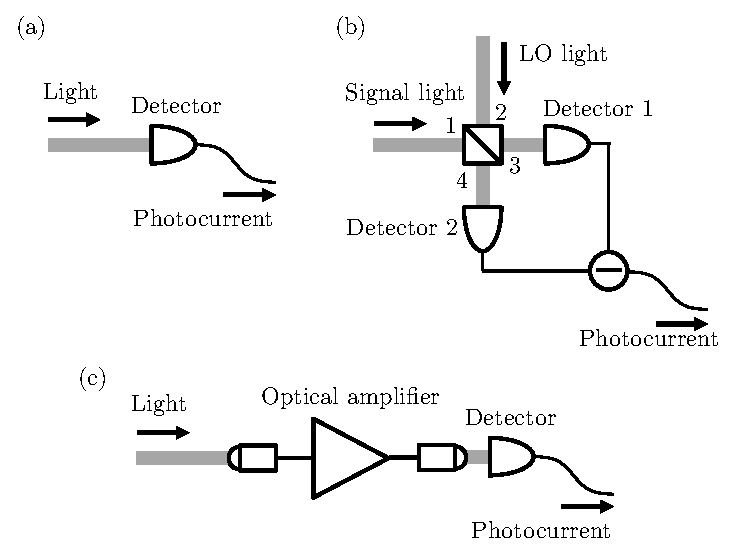
\includegraphics[width=9cm]{fig/1-1_photodetection.eps}
  \caption{代表的な光検出法。(a) 直接検出。(b) 干渉検出。(c) 光前置増幅。光を光ファイバ増幅器に入力し、光増幅後に直接検出する状況を記載している。}
  \label{fig:photodetection}
\end{figure}

%\begin{comment}
\subsection{直接検出}
まず、直接検出における電流と光パワーの関係を求めよう。光パワーを$P$、光子エネルギーを$\hbar \omega$とすると、単位時間あたりに到来する光子数は$P/\hbar \omega$である。入射した光子のうち電子に変換される割合を量子効率といい、$\eta$で表すと、単位時間あたりに発生する伝導電子の数は$\eta P/\hbar \omega$個である。したがって、電荷素量を$q = 1.602 \times 10^{-19} \ \mathrm{[C]}$とすれば、検出器の出力電流は次式で与えられる。
\begin{equation}
	I = \frac{\eta q P}{\hbar \omega}
	\nonumber
\end{equation}
ここで、$I/P = \eta q / \hbar \omega$は\textbf{光電変換効率}\index{こうでんへんかんこうりつ@光電変換効率}と呼ばれる。$\hbar \omega / q$は光子エネルギーをeVで表した値である。光通信波長である1.55 \ \textmu m では光子エネルギーは約0.8 eVである。また、典型的なフォトダイオードの量子効率は90\%程度であるから、この波長帯における光電変換効率は1.1 A/W程度である\footnote{1.5 \ \textmu m帯の光検出に用いられるInGaAsフォトダイオードのカタログを見てみると良い。Googleで``InGaAs pd''というキーワードで検索するといくつか見つかる。}。すなわち、1 mWの光を入力すると約1.1 mAの光電流が得られる。

ひとつの光子が入射した時に、多数の伝導電子が発生するタイプの検出器もあり、なだれフォトダイオード、光電子増倍管などが知られている\footnote{電子の増倍作用を用いたイメージセンサとして、EM-CCD (electron multiplying charge coupled device)も最近登場し、微弱光のイメージングに使われる。}。これは電子の増倍作用を用いて電流信号を大きくすることで検出器そのものの雑音の影響を相対的に小さく抑えることができるため、微弱光の検出に使われる\footnote{これらは増倍のプロセスが確率的であるため、信号対雑音比が3 dB程度低下する。}。

\subsection{干渉検出}

図\ref{fig:photodetection}(b)は典型的な干渉検出の模式図である。信号光と局発光をビームスプリッタで重ね合わせ、ビームスプリッタの2つの出力をそれぞれ別のフォトダイオードで検出する。これらのフォトダイオードが出力する光電流の差分を取る。この測定法を\textbf{バランスド検出法}という。信号光と局発光の周波数をそれぞれ$\omega + \Delta \omega, \omega$とするとき、$\Delta \omega = 0$の場合を\textbf{ホモダイン検出}、$\Delta \omega \neq 0$の場合を\textbf{ヘテロダイン検出}という\footnote{これらの言葉は、電気回路においてミキサを用いて周波数変換を行う場合と対応している。}。

バランスド検出法における出力信号は以下のように求めることができる。信号光と局発光の複素振幅をそれぞれ$\alpha, \beta$としよう。ただし、$|\alpha|^2, |\beta|^2$がそれぞれ時間$\tau$あたりの光子数になるように定義する。また、$\Delta \omega \ll \omega$であり、信号光と局発光の光子エネルギーの差は無視できるものとする\footnote{この仮定を置かないと信号光と局発光の電場の足し引きができない。}。この時、信号光と局発光の解析信号\footnote{電界$E(t)$を$E(t)=\mathrm{Re} \ E_0 e^{-i\omega t}$と書くとき、$E_0$を複素振幅といい、$E_0 e^{-i\omega t}$を解析信号という。つまり、解析信号とは、周波数が正の成分のみから構成されていて、その実部を取ると、実信号になるもの。}は
\begin{equation}
\begin{aligned}
	a(t) &= \alpha e^{-i(\omega + \Delta \omega)t}\\
  	b(t) &= \beta e^{-i\omega t}
\end{aligned}\label{eq:complex_amplitude}
\end{equation}
と表せる。ビームスプリッタのポート1および2にそれぞれ信号光および局発光を入力するときの、ポート3, 4から出力される光の解析信号をそれぞれ$a', b'$とすると、
\begin{equation}
\begin{aligned}
  a' &= \frac{1}{\sqrt 2}(a - b)\\
  b' &= \frac{1}{\sqrt 2}(a + b)
\end{aligned}\label{eq:BS_complex_amplitude}
\end{equation}
と表せる。$a'$の式の右辺で$b$の符号がマイナスになっているのは、ポート2からポート4に固定端反射が生じると仮定したためである\footnote{ポート1から3、もしくはポート2から4のどちらが固定端反射もしくは解放端反射かは、最終的な結果の位相に影響するだけで、全体の結論に大きな影響は及ぼさない。また、後で説明するように、ビームスプリッタを結合導波路として考える場合は、結合する側が$i$倍される。}。式(\ref{eq:BS_complex_amplitude})は行列を用いて
\begin{equation}
  \left( \begin{array}{c}
  	A' \\ B'
  \end{array}
  \right) =
  \frac{1}{\sqrt 2}\left( \begin{array}{r r} 
  	1 & -1 \\ 1 & 1
 \end{array}
	\right)
	\left( \begin{array}{c}
		A \\ B
	\end{array} \right)
	\label{eq:beamsplitter_matrix}
\end{equation}
と書くこともできる\footnote{この行列がユニタリであることは、光パワーの損失がないことに対応している。}。

ポート3, 4から出力される光を検出器1, 2で受光し、その光電流をそれぞれ$I_1, I_2$とすると、
\begin{equation}
\begin{aligned}
  I_1 &= \frac q \tau |a'|^2 = \frac{q}{\tau}\left|\frac{1}{\sqrt 2} (a - b)\right|^2\\
  I_2 &= \frac q \tau |b'|^2 = \frac{q}{\tau}\left|\frac{1}{\sqrt 2} (a + b)\right|^2
\end{aligned}
\end{equation}
を得る。したがって、
\begin{equation}
\begin{aligned}
  I_2 - I_1 &= \frac{q}{\tau}(ab^* + a^* b)\\
  &= 2qB(\alpha \beta^* e^{-i\Delta\omega t} + \alpha^* \beta e^{i\Delta\omega t})\\
  &= 4qB|\beta|\left\{\mathrm{Re} \  (\alpha e^{-i\phi}) \cos \Delta \omega t + \mathrm{Im} \ (\alpha e^{-i\phi}) \sin \Delta \omega t\right\}
\end{aligned}\label{eq:output_of_balanced_detector}
\end{equation}
ただし、$B = 1/2\tau$はナイキスト周波数である。また、$\beta = |\beta|e^{i\phi}$とおいた。

式(\ref{eq:output_of_balanced_detector})より、$\Delta \omega = 0$であれば$I_2 - I_1 = 4qB|\beta| \mathrm{Re} \ (\alpha e^{-i\phi})$であるから、$\alpha$の複素振幅の$\beta$の位相を基準とする軸への射影を計測することが可能であることがわかる。これがホモダイン検出である。

また、$\Delta \omega \neq 0$であれば、光電流には周波数$\Delta \omega$の正弦波が発生することがわかる。この$\cos$成分と$\sin$成分を求めることで、$\alpha$の複素振幅を求めることが可能である。これがヘテロダイン検出である。

\section{光計測における雑音}\label{section:1.2}

ここでは、光計測における基本的な雑音である、ショット雑音と熱雑音についてまとめておこう。また、ホモダインやヘテロダインにおけるショット雑音の影響と、前置増幅を行った場合の雑音についても考えてみよう。熱雑音を回避した場合、信号対雑音比がおよそ光子数のオーダになることが見て取れるであろう。

\subsection{ショット雑音}
まず、天下り的に、光を計測した時に光子が検出器に確率的に到来すると仮定しよう。この時、よく知られているように、光子の個数$k$の分布はポアソン分布に従い、その確率分布は
\begin{equation}
	p(k) = \frac{\lambda^k e^{-\lambda}}{k!}
\end{equation}
で与えられる。ただし、$\lambda$は平均の光子の個数である。

ポアソン分布の特徴として、個数の分散と平均値が等しいことが知られている。このことは、次式によって確かめられる。
\begin{equation}
\begin{aligned}
	V[p(k)] &= \sum_k{(k-\lambda)^2}p(k) = \sum_k{k^2 p(k) - 2\lambda k p(k) + \lambda^2 p(k)} = \sum_k{k^2 p(k) - \lambda^2} \\
	&=\sum_k{k\lambda p(k-1) - \lambda^2} = \lambda\sum_k{\left\{ (k-1)p(k-1) + p(k-1)\right\}}-\lambda^2 = \lambda(\lambda + 1) - \lambda^2 = \lambda
\end{aligned}
\end{equation}
ただし、$\sum_k p(k) = 1$、$\sum_k kp(k) = \lambda$を用いた。

このため、光子数を信号$S$、光子数の標準偏差を雑音$N$とし、信号パワーと雑音パワーの比を信号対雑音比(SNR)とすると、
\begin{equation}
	\mathrm{SNR} = (S/N)^2 = \lambda^2/\lambda = \lambda
\end{equation}
となり、平均の光子数が大きいほどSNRが高くなることがわかる。

このような光子数の揺らぎに由来する光電流の雑音を\textbf{ショット雑音}\index{しょっとざつおん@ショット雑音}という。ショット雑音を電流で表すときは、スペクトル密度で表すことが多い。このために、ある短い時間$\tau$を考え、この時間内に到来する光子数の平均が$\lambda$であるとしよう。このとき$I = q\lambda / \tau$である。ショット雑音の電流を実効値もしくは自乗平均平方根(RMS: root mean square)で表すと、
\begin{equation}
	\begin{aligned}
		I_{\mathrm{shot}} = q\sqrt{\lambda}/\tau = q\sqrt{\frac{I\tau}{q}}/\tau = \sqrt{\frac{qI}{\tau}}
	\end{aligned}
\end{equation}

検出器の帯域を$B$とすると、サンプリング定理より、時間$\tau$ごとに検出する光子数が独立になるためには$B = 1 / 2\tau$の帯域が必要であるから、ショット雑音による電流雑音の実効値は次式で与えられる。
\begin{equation}
	\begin{aligned}
		I_\mathrm{shot}=\sqrt{2qIB}
	\end{aligned}
\end{equation}
なお、$I_\mathrm{shot}$の単位は$\mathrm{[A]}$である。

また、式(\ref{eq:complex_amplitude})と同様の定義を用い、信号光の複素振幅を$\alpha$としてショット雑音限界のSNRを表すと、次式のようになる。
\begin{equation}
  \mathrm{SNR} = I^2 / I_\mathrm{shot}^2 = I/2qB = 2qB|\alpha |^2/2qB = |\alpha|^2
\end{equation}
ただし、$I=q|\alpha|^2/\tau = 2qB|\alpha|^2$を用いた。$|\alpha|^2$は光子数を表すから、この式はショット雑音限界のSNRが光子数と一致することと対応している。

しかし、$\alpha$は連続量であり、離散的な整数である「光子数」と一致する、ということはどういうことであろうか。また、$\alpha$という複素数の位相は光子とどのように関係するのであろうか。これらの点は古典論の議論では明らかにならない。

\subsection{熱雑音}

図1.2(a)に示すように、光検出の際には光電流$I$を抵抗$R$に流し、抵抗の両端に現れる電圧$R I$を検出する場合が多い。抵抗があると、その両端には、実効値電圧
\begin{equation}
	v_\mathrm{th} = \sqrt{4k_\mathrm{B}TRB}
	\label{eq:Johnson_noise}
\end{equation}
を持つ雑音が発生することが知られている。ただし、$k_B$はボルツマン定数、$T$は抵抗の絶対温度、$B$は回路の帯域である。この雑音を\textbf{ジョンソン雑音}\index{じょんそんざつおん@ジョンソン雑音}、もしくは単に熱雑音という。熱雑音は光計測における信号対雑音比の低下要因となるため、熱雑音が光の雑音よりも小さく抑えられるように注意深く測定系を設計する必要がある。
\begin{figure}
  \centering
  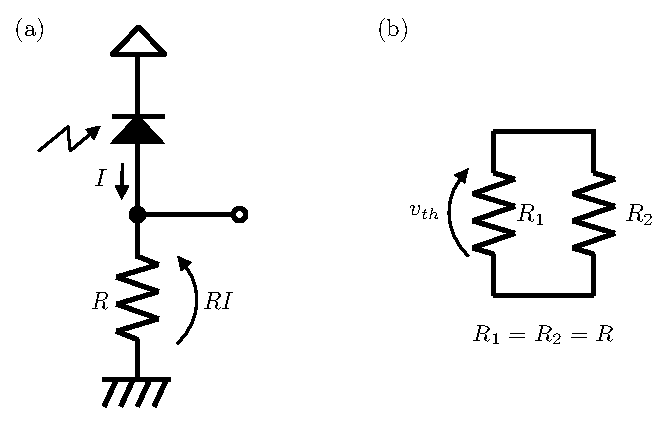
\includegraphics[width=7cm]{fig/1-2_PD_circuit.eps} 
  \caption{(a) 典型的な光検出回路。PDに逆バイアスをかけ、光電流$I$を負荷抵抗$R$に流すことで、負荷抵抗に現れる電圧$RI$を検出する。(b) ジョンソン雑音について考えるための仮想的な回路。}
  \label{fig:photodetector}
\end{figure}

ジョンソン雑音の式(式(\ref{eq:Johnson_noise}))を導出するために、図1.2(b)に示す回路を考えよう。抵抗1 ($R_1$)ともう一つの抵抗2 ($R_2$)を接続し、インピーダンスマッチングするように$R_1 = R_2 = R$とする。抵抗1の熱雑音が作る起電力を$v_{th}$とすると、回路一周の抵抗が$2R$であることから、起電力によって流れる電流は$v_{th}/2R$である。この時、この熱雑音が抵抗2に与えるパワーは$v_{th}^2/2R$となる。同様に、抵抗2から抵抗1にも同じパワーが与えられることで、抵抗1と抵抗2が熱平衡状態を保っている\footnote{抵抗1と抵抗2の温度が違う場合は、電気を介して熱の移動が生じる。}。

熱雑音を時間間隔$\tau$でサンプリングする\footnote{この表現はちょっとラフである。もう少し丁寧に表現すると、以下のようになる:熱雑音由来の電圧雑音に対して$-1/2\tau < f < 1/2\tau$までの周波数制限をかけたと仮定しよう。このとき、時間領域で時間間隔$\tau$ごとに離散的にサンプリングすることで電圧波形の情報を得ることができる。これらひとつひとつのサンプリング点が、雑音波形の自由度に対応し、それらにボルツマンエネルギー$k_B T$が分配される。}と、$B = 1/2\tau$までの情報を捉えることができる。各サンプリング間隔において起電力が行う仕事は$v^2_{th}\tau/2R$であり、これら全ての自由度に対してボルツマンエネルギー$k_BT$が分配されることから、次式が成り立つ。
\begin{equation}
v_\mathrm{th}^2\tau/2R = v_\mathrm{th}^2 / 4RB = k_\mathrm{B}T
\end{equation}
この式から式(\ref{eq:Johnson_noise})を得る。
%\footnote{1モードあたり$k_BT/2$ではなく$k_BT$のエネルギーを持つのは、振動子が位置と運動量の2つの自由度を持つため。}

\subsubsection{熱雑音とショット雑音の大きさの比較}
光検出において熱雑音とショット雑音のどちらが支配的かを意識しておくことは重要である。そのイメージを持つために、熱雑音とショット雑音が等しくなる条件を考えてみよう。この条件は、$RI_\mathrm{shot} = v_\mathrm{th}$と表される。この関係が成り立つときの$I$を$I'$とおくと、
\begin{equation}
	I' = 2\frac{k_\mathrm B T }{qR}
\end{equation}
を得る。$k_\mathrm{B}T/q$はボルツマンエネルギーをeVで表したものであり、室温($T$ = 300 K)において$26 \ \mathrm{meV}$である。

負荷抵抗を$R = 50 \ \Omega$とすれば、$I = 1 \ \mathrm{[mA]}$の時に熱雑音はショット雑音と等しくなる。また、これよりも強い光を計測する場合は$I$が大きくなりショット雑音が顕在化する。一方、弱い光を計測する時は、$I$が小さくなるため、熱雑音が支配的な雑音となる。ショット雑音、熱雑音はそれぞれ$R$、$\sqrt R$に比例するので、負荷抵抗を大きくすれば、熱雑音の影響を相対的に抑えることは可能である。その場合は、光検出器が有するキャパシタンス$C$による$RC$時定数が大きくなるため、回路の応答速度が制限を受けてしまう。

\subsection{干渉検出におけるショット雑音}
1.1節で述べたように、干渉検出法を用いることで光の複素振幅を計測することが可能である。それに加えて、LO光の強度を高めることで、検出器の熱雑音の影響を抑えて計測することも可能である。ここでは、LO光の強度を高め、ショット雑音が支配的となる状況における干渉検出のSN比について考えよう。

ダブルバランスド検出器による干渉検出における信号は式(\ref{eq:output_of_balanced_detector})で与えられる。ここで、LO光の位相を$\phi = 0$としよう。また、LO光が信号光より高強度であるとすると、ショット雑音の大きさはLO光の強度で決まると仮定できる\footnote{このことは量子論では成り立たず、ショット雑音は信号光で決まることが示される。}。LO光がビームスプリッタで2分割されることを考慮すると、各検出器の出力電流は
\begin{equation}
  I_1 \sim I_2 \sim \frac 1 2 \frac q {\tau} |\beta|^2 = qB|\beta|^2
\end{equation}
である。また、各検出器のショット雑音は
\begin{equation}
  \sqrt{2qI_1B} \sim \sqrt{2qI_2B} \sim \sqrt{2q^2B^2|\beta|^2} =\sqrt 2 qB|\beta|
\end{equation}
である。バランスド検出器は2つの検出器の信号の差を出力し、その際に独立な雑音の振幅は自乗和の平方根となる。このことから、バランスド検出器のショット雑音は
\begin{equation}
  I_\mathrm{shot} = 2qB|\beta|
  \label{eq:shot_noise_of_balanced_detector}
\end{equation}
となる。

ホモダインの場合の検出器の出力電流$I_\mathrm{homodyne}$は、式(\ref{eq:output_of_balanced_detector})において$\Delta \omega = 0$と置くことで
\begin{equation}
  I_\mathrm{homodyne} = 4qB|\beta|\mathrm{Re} \ \alpha
\end{equation}
で与えられる。したがって、ホモダインの信号対雑音比は次式のようになる。
\begin{equation}
  \mathrm{SNR_{homodyne}} = I_\mathrm{homodyne}^2/I_\mathrm{shot}^2 = 4(\mathrm{Re} \ \alpha)^2
\end{equation}
このようにホモダイン信号のSN比は信号光のエネルギーで決まり、局発光の強度にはよらない。

ヘテロダインの場合、話が少し複雑である。まず、ヘテロダイン信号をcos成分とsin成分にわけ、
\begin{equation}
  I_\mathrm{cos} = 4qB|\beta|(\mathrm{Re} \ \alpha) \cos\Delta\omega t
\end{equation}
\begin{equation}
  I_\mathrm{sin} = 4qB|\beta|(\mathrm{Im} \ \alpha) \sin\Delta\omega t
\end{equation}
と表そう。これらの2乗の時間平均を取ると、
\begin{equation}
  \overline{I_\mathrm{cos}^2} = (4qB|\beta|\mathrm{Re} \ \alpha)^2 \frac{1}{2}\overline{(1+\cos 2\Delta \omega t)} = 8(qB|\beta|\mathrm{Re} \ \alpha)^2
\end{equation}
\begin{equation}
  \overline{I_\mathrm{sin}^2} = (4qB|\beta|\mathrm{Im} \ \alpha)^2 \frac{1}{2}\overline{(1-\cos 2\Delta \omega t)} = 8(qB|\beta|\mathrm{Im} \ \alpha)^2
\end{equation}
である。したがって、それぞれの信号対雑音比は、次式で与えられる\footnote{ここでのショット雑音の議論はだいぶ途中を省略している。バランスド検出器の出力に含まれるショット雑音のうち、$\Delta \omega/2\pi - B$から$\Delta \omega/2\pi + B$、すなわち帯域$2B$の周波数成分を考慮する必要があるが、ここにはcos成分とsin成分が含まれるので、cos成分のみのショット雑音は式(\ref{eq:shot_noise_of_balanced_detector})と等しくなる。}。
\begin{equation}
  \overline{I_\mathrm{cos}^2}/I_\mathrm{shot}^2 = 2(\mathrm{Re} \ \alpha)^2
\end{equation}
\begin{equation}
  \overline{I_\mathrm{sin}^2}/I_\mathrm{shot}^2 = 2(\mathrm{Im} \ \alpha)^2
\end{equation}
これはホモダインにおける信号対雑音比の半分である。

以上の議論から、ホモダインでは複素振幅の実部もしくは虚部しか計測できないが、ヘテロダインでは実部と虚部の両方を検出できる代わりに、信号対雑音比がホモダインの半分となること、すなわち3 dB低下することがわかる。

\subsection{光前置増幅における増幅器雑音}

光前置増幅において、信号対雑音比を制限するのは、光増幅器が発生するASE (amplified spontaneous emission)、すなわち「増幅された自然放出光」である。ASEのパワーは、単一偏光あたり
\begin{equation}
	P_0 = n_\mathrm{sp}\hbar \omega (G-1)\Delta f
\end{equation}
で与えられることが知られている。ただし、$G$は増幅器利得、$\Delta f$は光の帯域幅である。また、$n_\mathrm{sp}$は自然放出係数と呼ばれ、レーザー媒質の反転分布が完全でない時や、光損失が存在する場合に1より大きな値をとる。
なお、多くの場合、光増幅器は縦横両方の偏光でASEを発生するので、両偏光のASEパワーの和は
\begin{equation}
	P_\mathrm{ASE} = 2n_\mathrm{sp}\hbar \omega (G-1)\Delta f
\label{eq:ASE_power}
\end{equation}
となる。

ここで、入力光パワーを$P_\mathrm{in}$とする。また、ASEはcos成分、sin成分に分けられる。ASE雑音のうちcos成分のみに注目し、そのパワーを$P_\mathrm{ASE1}$とすると、これは単一偏光のASEパワー$P_0$の半分となるから、
\begin{equation}
  P_\mathrm{ASE1} = \frac{1}{2}n_{sp}\hbar\omega(G-1)2B = n_{sp}\hbar\omega(G-1)B 
  %= \frac{n_{sp}(G-1)}{2\tau}\hbar \omega
\end{equation}
である。ただし、$\Delta f = 2B$としたのは、信号光の周波数を中心として周波数帯域$\pm B$に含まれるASEが雑音に寄与すると考えたためである。このASEの電界が信号光に重ね合わされると、光パワーは次式のように変化する。
\begin{equation}
  \left(\sqrt{GP_{in}} \pm \sqrt{P_\mathrm{ASE1}}\right)^2 = GP_{in} \pm 2\sqrt{GP_{in}P_\mathrm{ASE1}} + P_\mathrm{ASE1}
\end{equation}
右辺第2項は信号光とASEの干渉による強度変化であり、\textbf{シグナル-ASEビート雑音}\index{しぐなるASEびーとざつおん@シグナル-ASEビート雑音}と呼ばれる。このシグナル-ASEビート雑音が支配的と仮定すれば、増幅後のSNRは次式で与えられる。

\begin{equation}
  \mathrm{SNR} = \left(\frac{GP_{in}}{2\sqrt{GP_{in}P_\mathrm{ASE1}}}\right)^2 = \frac{GP_{in}}{4P_\mathrm{ASE1}}=\frac{GP_{in}}{4n_{sp}\hbar\omega(G-1)B}\to \frac{1}{2n_{sp}}\frac{P_{in}}{2\hbar\omega B}
\end{equation}
ここで、$\frac{P_{in}}{2\hbar\omega B}$は時間$\tau = 1/2B$に含まれる光子数であり、増幅前のショット雑音限界のSNRと等しい。したがって、光増幅によって、信号対雑音比は$1/2n_{sp}$倍に低下することがわかる。信号対雑音比の低下量である$2n_{sp}$を\textbf{雑音指数}(noise figure, NF)という。特に、$n_{sp} = 1$のときの雑音指数(2、もしくは3 dB)を量子限界の雑音指数という。典型的な光ファイバ増幅器の雑音指数は5 - 6 dBであることが多い。

\subsection{光計測におけるその他の雑音}
ここまでで説明したショット雑音、熱雑音、増幅器雑音は、光計測における基本的な雑音源であるが、他にも雑音源は無数に存在する。ここでは過剰雑音と$1/f$雑音について簡単に説明しておこう。

\subsubsection{過剰雑音}
光がショット雑音よりも大きな雑音を有する場合、それらをまとめて過剰雑音という。過剰雑音の原因は多岐にわたるが、光源の安定性の低さによるものや、自然放出光の重畳によるものなどが挙げられる。ASEは過剰雑音の一種である。

\subsubsection{1/f雑音}
能動素子や光源は低周波数において大きな揺らぎを持ち、その揺らぎのパワースペクトルが$1/f$に比例する場合が多いことが知られている。このことを$1/f$雑音という。ショット雑音や熱雑音が周波数に依存しないホワイトノイズであるのに対して、$1/f$雑音は低周波数で顕著になる。このため、長時間の平均化を行った際の雑音要因になりうる。

同様のノイズに、$1/f^2$雑音もある。これは、ホワイトノイズにローパスフィルタをかけたものである。

%\begin{comment}

\section{量子光学の必要性}
以上の議論では、ショット雑音や増幅器雑音を現象論として与えた。これらの式を用いれば、それを元に光信号の信号対雑音比の評価を行うことができる。一方、なぜ、どういう場合にこれらの式が成り立つのか、という問いに答えるには、その背後にある物理を考える必要がある。それが量子光学である。

	
量子光学では、光の場を多数の空間モードおよび時間/周波数モードに分解し、ひとつひとつのモードを放物線ポテンシャルの量子力学で表す。複数のモードの量子状態を規定し、それに対してある物理量の測定を行うことで、物理量の期待値およびその揺らぎを求める。このような枠組みのもとで、光子の集まりとしての光の振る舞いを記述することができる。

\section{まとめ}
本章では、代表的な光計測法である直接検出法、干渉検出法や、光前置増幅法について原理を述べるとともに、ショット雑音限界のSNRがほぼ光子数で決まることを述べた。

%\end{comment}

\chapter{調和振動子の量子力学}

前章の議論では、ショット雑音や増幅器雑音を現象論として与えた。これらの式を用いれば、それを元に光信号の信号対雑音比の評価を行うことができる。一方、なぜ、どういう場合にこれらの式が成り立つのか、という問いに答えるには、その背後にある物理を考える必要がある。それが量子光学である。
	
量子光学では、光の場を多数の空間モードおよび時間/周波数モードに分解し、ひとつひとつのモードを量子力学的な調和振動子とみなす。複数のモードの量子状態を規定し、それに対してある物理量の測定を行うことで、物理量の期待値およびその揺らぎを求める。このような枠組みのもとで、光子の集まりとしての光の振る舞いを記述することができる。

本章では、調和振動子の量子力学の基本についておさらいをしておこう。


\section{調和振動子}
ばねと重りからなる、減衰のない調和振動子を考え、そのばね定数を$k$、重りの質量を$m$としよう。振動子の共振角周波数は$\omega = \sqrt{k/m}$である。また、重りの位置の平衡点からのずれを$q$と表す。ここで、ばねのエネルギーを
\begin{equation}
	\frac{k}{2}x^2 \equiv \frac{1}{2}(\omega q)^2
\end{equation}
と表し、振動子の運動エネルギーを
\begin{equation}
	\frac{m}{2}\left(\frac{dx}{dt}\right)^2\equiv\frac{1}{2}p^2
\end{equation}
と表そう\footnote{本来ならばばねのエネルギーは$\frac 1 2 m\omega_0^2 x^2$、運動エネルギーは$p^2/2m$とするべきだが、この後で調和振動子を光の場に対応させる際に、光には重さがないのでつじつまが合わないため、$m = 1$とし、光には$\hbar k$の運動量があることを前提条件として話を進める。}。
図\ref{fig:classical_phase_space}(a)に示すように、$q$を横軸に、$p$を縦軸として振動子の状態を表す。このような2次元平面を位相平面という。振動子の運動エネルギーとポテンシャルエネルギーの和は一定であることから、時間発展とともに右回りの円の軌跡を描く。

あとで示すように、量子力学では位置や運動量が広がりを持つ確率分布として与えられる。イメージとしては図\ref{fig:classical_phase_space}(b)のようになる。ただし、この図はあくまでイメージであって、そのまま信じてはいけない。揺らぎの様子は、位置だけを測定するのか、位置と運動量を同時に測定するのかによって変わって来る。また、量子力学では、位相が確定しない状態等、様々な状態が存在しうる。

\begin{figure}
  \centering
  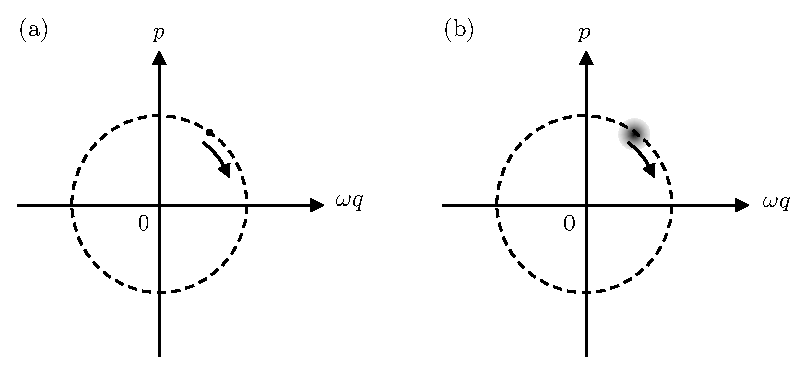
\includegraphics[width=9cm]{fig/2-1_phase_space.eps} 
  \caption{位相平面における調和振動子の位置と運動量の時間発展。(a) 古典的な調和振動子。(b) 量子的な調和振動子。}
  \label{fig:classical_phase_space}
\end{figure}


\section{シュレディンガー方程式とハイゼンベルグの運動方程式}
量子力学では、系の量子状態を状態ベクトル\footnote{波動関数、量子状態とも同じ。}で表すとともに、位置$q$や運動量$p$をエルミート演算子$\hat q, \hat p$で表すことでシュレディンガー方程式を立て、それを解いていく。詳細は付録を参照してほしい。なぜ演算子で表すのかというと、位置や運動量に揺らぎ、もしくは不確定性があるからである。調和振動子がある量子状態にあったとすると、位置も運動量も確率分布としてしか知ることはできない。このとき、量子状態から確率分布を抽出する操作を、演算子で表現する。また、演算子は位置や運動量のような物理量を表す際だけでなく、量子状態に変化を与える際にも用いる。

本節では、シュレディンガー方程式が状態ベクトルの時間変化を記述する方程式であることを説明する。このように状態ベクトルを時間発展させていく描像を「シュレディンガー描像」という。また、時間発展操作を加える演算子である時間発展演算子を導入する。
さらに、状態ベクトルを時間発展させるのではなく、演算子を時間発展させる計算方法である「ハイゼンベルグ描像」について説明するとともに、演算子の時間発展を表す方程式であるハイゼンベルグの運動方程式を導入する。

後の章で説明するように、時間発展演算子やハイゼンベルグの運動方程式は、時間発展以外の操作にも使うことができる。これによって、光の発生、検出、増幅等の計算が極めてシンプルになる。一方で、これらの計算を理解する上で、シュレディンガー描像のことを表しているのか、ハイゼンベルグ描像のことを表しているのかをきちんと押さえておくことが重要である。

\subsection{シュレディンガー方程式と時間発展演算子}
時間とともに変化する状態ベクトル$\ket{\Psi(t)}$の時間変化を記述する方程式
\begin{equation}
  i\hbar \frac{d}{dt}\ket{\Psi(t)} = \hat H \ket{\Psi(t)}
  \label{eq:Schrodinger_equation}
\end{equation}
を\textbf{シュレディンガー方程式}という。この式の左辺は、状態ベクトルの時間微分を$i\hbar$倍したものである。右辺は、エネルギーを表す演算子(ハミルトニアン)を状態ベクトルに作用させたものである。

$\hat H$が時間変化しない場合、式(\ref{eq:Schrodinger_equation})は簡単に解くことができる。まず、微分を微小時間$\Delta t$での差分に置き換えると、
\begin{equation}
  	\ket{\Psi(\Delta t)} - \ket{\Psi(0)} \sim \frac{\Delta t}{i\hbar}\hat H \ket{\Psi(0)}
\end{equation}
より、
\begin{equation}
  \ket{\Psi(\Delta t)} \sim \left( 1 + \frac{\hat H}{i\hbar}\Delta t\right)\ket{\Psi(0)}
\end{equation}
であるから、次式を得る。
\begin{equation}
  \ket{\Psi(N\Delta t)}\sim \left(1 + \frac{\hat H}{i\hbar}\Delta t\right)^N\ket{\Psi(0)}
\end{equation}
ここで、$t = N\Delta t$として$N \to \infty$の極限を取ると、シュレディンガー方程式の解として次式が得られる。
\begin{equation}
  \ket{\Psi(t)} = \exp \left( \frac{\hat H}{i\hbar}t \right) \ket{\Psi(0)}
  \label{eq:Schrodinger_solution}
\end{equation}
である。ここで、$\hat H$の固有ベクトルを$\ket{\Psi_k}$、エネルギー固有値を$E_k$とすれば、$\hat H \ket{\Psi_k (0)}=E_k\ket{\Psi_k (0)}$であるから、これを(\ref{eq:Schrodinger_solution})に代入すると
\begin{equation}
  \ket{\Psi_k(t)} = \exp\left(-i\frac{E_k}\hbar t\right)\ket{\Psi_k(0)}
  \label{eq:time_evolution_of_steady_state}
\end{equation}
を得る。すなわち、式(\ref{eq:Schrodinger_solution})は、各エネルギー固有状態を、各エネルギーに対応する周波数$\omega_k = E_k / \hbar$で時間とともに位相回転させている。これはドブロイの関係式$E = \hbar \omega$を表したものである、と考えることもできる。

ここで、式(\ref{eq:Schrodinger_solution})に現れる
\begin{equation}
  \hat U(t) \equiv \exp \left( \frac{\hat H}{i\hbar} t \right)
\end{equation}
を\textbf{時間発展演算子}といい、$\ket{\Psi(t)} = \hat U(t) \ket{\Psi(0)}$である。また、$\hat U ^\dagger (t) = \hat U(-t)$であるから、$\hat U^\dagger \hat U = \pmb 1$となり、時間発展演算子がユニタリであることがわかる
\footnote{時間発展演算子がユニタリであることは、波動関数のノルムを変化させない、すなわち、粒子の存在確率を変化させないことに対応している
。これは、エルミート演算子であるハミルトニアンの固有値(エネルギー固有値)が実数であるために、式(\ref{eq:time_evolution_of_steady_state})において各固有ベクトルの振幅が時間とともに変化しないこととも対応している。}。
%\footnote{$\hat H$が時間とともに変化する場合も、時間発展演算子を求めることができ、やはりユニタリ行列となる。}

\subsection{シュレディンガー描像とハイゼンベルグ描像}
振動子の変位のように、時間とともに変化する物理量の期待値を計算することを考えよう。この時、状態ベクトルが時間とともに変化するとして考えると、その期待値$\braket{\hat A}$は
\begin{equation}
  \braket{\hat A} = \braket{\Psi(t)|\hat A | \Psi(t)}
  \label{eq:Schrodinger_picture}
\end{equation}
として計算することができる\footnote{付録のA.2節を参照のこと。}。

一方、状態ベクトルに対し、時間発展演算子を作用させることで時間発展を表すと、
\begin{equation}
  \braket{\Psi(t)|\hat A|\Psi(t)} = \braket{\Psi(0)|\hat U^\dagger(t) \hat A \hat U(t) | \Psi(0)} \equiv \braket{\Psi(0) | \hat A_\mathrm H(t) | \Psi(0)}
  	\label{eq:Heisenberg_picture}
\end{equation}
と表すことができる。

式(\ref{eq:Schrodinger_picture})のように、時間とともに状態ベクトルを変化させて時間変化を考えることを、\textbf{シュレディンガー描像}\index{しゅれでぃんがーびょうぞう@シュレディンガー描像}という。一方、式(\ref{eq:Heisenberg_picture})のように物理量の演算子を変化させることで時間変化を考えることを\textbf{ハイゼンベルグ描像}\index{はいぜんべるぐびょうぞう@ハイゼンベルグ描像}という。

シュレディンガー描像は、波動関数の時間発展を直感的に捉える上で有用である。一方、光の量子論では、ハイゼンベルグ描像を用いて、演算子を変化させて様々な状況を計算することが多用される。

ハイゼンベルグ描像では、時間発展を以下のようにして計算する。
\begin{equation}
\begin{aligned}
  \frac{d}{dt}\hat A_\mathrm H (t) &= \left( \frac d {dt} \hat U^\dagger (t)\right) \hat A \hat U(t) + \hat U^\dagger \hat A \left( \frac{d}{dt}\hat U(t) \right)\\
	&= \frac{-\hat H}{i\hbar} \hat U^\dagger (t)\hat A\hat U(t) + \frac{1}{i\hbar}\hat U^\dagger(t) \hat A \hat U(t) \hat H\\
	&= \frac{i}{\hbar}\left( \hat H \hat A_\mathrm H(t) - \hat A_\mathrm H(t) \hat H \right) = \frac{i}{\hbar}\left[ \hat H, \hat A_\mathrm H \right]
\label{eq:Heisenberg_equation_of_motion}
\end{aligned}
\end{equation}
ただし、$\hat H$が時間と共に変化しないことを仮定した。また、$\hat H$と$\hat U$が交換可能であることを用いた\footnote{$\hat U$をテーラー展開すれば、$\hat H$の多項式で表せる。このことから$\hat U$と$\hat H$が交換可能であることがわかる。}。この式(\ref{eq:Heisenberg_equation_of_motion})を\textbf{ハイゼンベルグの運動方程式}\index{はいぜんべるぐのうんどうほうていしき@ハイゼンベルグの運動方程式}という。

\section{調和振動子のシュレディンガー方程式とその解}
ここまでで述べてきたように、古典的な調和振動子は、位置$q$と運動量$p$の平面(位相平面)における回転運動として表される。また、量子論では、位置と運動量を演算子$\hat q$と$\hat p$で表す。調和振動子では、計算をシンプルにするために、消滅・生成演算子$\hat a, \hat a^\dagger$を導入する。本節では、消滅・生成演算子を用いて、調和振動子の解を求める。光の量子論では、この生成・消滅演算子が重要な役割を果たす。

\subsection{調和振動子のハミルトニアンと生成・消滅演算子}
調和振動子のエネルギーは、位置エネルギー$\frac{1}{2}(\omega \hat q)^2 $と運動エネルギー$\frac{1}{2}\hat p^2 $の和である。エネルギー演算子であるハミルトニアンは、
\begin{equation}
  \hat H = \frac{1}{2}(\omega \hat q)^2 + \frac 1 2 \hat p^2
\end{equation}
と表される。ここで、式を簡略化するために、規格化した位置および振幅の演算子$\hat P, \hat Q$を用いて、
\begin{equation}
  \hat H = \frac 1 2 \hbar \omega (\hat Q ^2 + \hat P^2)
\end{equation}
と表そう。このような置き換えは、
$\hat Q = \sqrt \frac{\omega}{\hbar} \hat q$, 
$\hat P = \frac{1}{\sqrt{\hbar \omega}}\hat p$と
おくことによって可能である。また、この$\hat Q$, $\hat P$に対しては以下の交換関係が成り立つ。
\begin{equation}
  [\hat Q, \hat P] = \left[\sqrt{\frac{\omega}{\hbar}}\hat q, \frac{1}{\sqrt{\hbar \omega}}\hat p \right] = \frac{1}{\hbar}[\hat q, \hat p] = i
  \label{eq:commutation_Q_P}
\end{equation}
ただし、$[\hat q, \hat p] = i\hbar$は量子論の要請である\footnote{詳細は\ref{section:commutation}節を参照されたい。}。

ここでさらに、複素振幅の演算子である$\hat a$を次式で定義する。
\begin{equation}
  \hat a = \frac{1}{\sqrt 2}(\hat Q + i\hat P)
  \label{eq:annihilation_operator}
\end{equation}
このとき、$\hat a$のエルミート共役は次式で与えられる。
\begin{equation}
  \hat a^\dagger = \frac{1}{\sqrt 2}(\hat Q - i\hat P)
  \label{eq:creation_operator}
\end{equation}
ただし、ここでは$\hat Q$および$\hat P$がエルミートであること、すなわち$\hat Q^\dagger = \hat Q$, $\hat P^\dagger = \hat P$であることを用いた。

$\hat a$は\textbf{消滅演算子}、$\hat a^\dagger$は\textbf{生成演算子}と呼ばれ、以下のような様々な性質を持つ。
\subsubsection{非エルミート性}
明らかに$\hat a^\dagger \neq \hat a$であるから、$\hat a^\dagger$、$\hat a$はエルミート演算子ではない。このため、$\hat a$は量子力学において誤差なく測定可能な物理量ではない。一方、後で議論するように一定の誤差を許せば、$\hat a$が表す物理量(複素振幅)を測定することは可能である。

\subsubsection{交換関係}
生成・消滅演算子は交換せず、次式が成り立つ。
\begin{equation}
  [\hat a, \hat a^\dagger] = \hat a \hat a^\dagger - \hat a^\dagger \hat a = 1
\end{equation}
証明は以下の通り。
式(\ref{eq:creation_operator}), (\ref{eq:annihilation_operator}), (\ref{eq:commutation_Q_P})を用いて次式を得る。
\begin{equation}
\begin{aligned}
  \left[\hat a , \hat a^\dagger\right] &= \frac{1}{2}\left\{(\hat Q + i\hat P)(\hat Q - i\hat P) - (\hat Q - i\hat P)(\hat Q + i\hat P)\right\} \\
  &= i(\hat P\hat Q - \hat Q\hat P) = -i[\hat Q, \hat P] = 1
\end{aligned}
\end{equation}

\subsubsection{生成・消滅演算子によるハミルトニアンの表現}
$\hat Q$, $\hat P$で表される演算子は全て生成・消滅演算子で表すことができる。実際、調和振動子のハミルトニアンは次式のように書ける。
\begin{equation}
  \hat H = \frac{\hbar \omega}{2}(\hat Q^2 + \hat P^2) = \frac{\hbar \omega}{2}(\hat a^\dagger \hat a + \hat a \hat a^\dagger) = \hbar \omega\left(\hat a^\dagger \hat a + \frac 1 2\right)
\end{equation}
ただし、$\hat Q = (\hat a + \hat a^\dagger)/\sqrt 2$, $\hat P = (\hat a - \hat a^\dagger) / i\sqrt 2$を用いた。

また、$\hat H$と$\hat a$, $\hat a^\dagger$は以下のような交換関係を有する。
\begin{equation}
\begin{aligned}
  \left[\hat H, \hat a\right] &= [\hbar \omega (\hat a^\dagger \hat a + 1/2), \hat a] = \hbar \omega [\hat a^\dagger \hat a, \hat a] = \hbar \omega (\hat a^\dagger \hat a \hat a - \hat a \hat a^\dagger \hat a)\\ 
  &= \hbar \omega (\hat a^\dagger \hat a \hat a - (\hat a^\dagger \hat a + 1) \hat a) = -\hbar\omega \hat a
\end{aligned}
\end{equation}
\begin{equation}
  \begin{aligned}
  	\left[\hat H, \hat a^\dagger \right] &= [\hbar \omega (\hat a^\dagger \hat a + 1/2), \hat a^\dagger] = \hbar \omega [\hat a^\dagger \hat a, \hat a^\dagger] = \hbar \omega (\hat a^\dagger \hat a \hat a^\dagger - \hat a^\dagger \hat a^\dagger \hat a)\\ 
  &= \hbar \omega (\hat a^\dagger (\hat a^\dagger \hat a + 1) - \hat a^\dagger \hat a^\dagger\hat a) = \hbar\omega \hat a^\dagger
  \end{aligned}
\end{equation}
これらの交換関係は、ハイゼンベルグ描像における時間発展の計算に用いられる。

\subsection{消滅演算子の実部および虚部の演算子}
$\hat a$の実部および虚部の演算子を次式で定義する。
\begin{equation}
  \begin{aligned}
  	\hat a_1 &\equiv \frac 1 2 (\hat a + \hat a^\dagger) = \frac 1 {\sqrt 2} \hat Q\\
  	\hat a_2 &\equiv \frac 1 {2i} (\hat a - \hat a^\dagger) = \frac 1 {\sqrt 2} \hat P
  \end{aligned}
\end{equation}
これらはいずれもエルミートである\footnote{$\hat a_1^\dagger = \hat a_1, \hat a_2^\dagger = \hat a_2$であることは定義からすぐわかる。}。このことから、$\hat a_1$および$\hat a_2$は固有状態と固有ベクトルを有し、物理量の計測が可能である。

ただし、$\hat a_1$と$\hat a_2$を同時に測定することはできない。これは、
\begin{equation}
  \left[ \hat a_1, \hat a_2\right] = \frac 1 2 [\hat Q, \hat P] = \frac i 2
\end{equation}
であることによる。


\subsection{生成・消滅演算子の時間発展}
前節で述べたように、ハイゼンベルグ描像では演算子が時間発展する。ハイゼンベルグの運動方程式より、
\begin{equation}
  \frac{d}{dt}\hat a(t) = \frac{i}{\hbar}[\hat H, \hat a(t)] = -i\omega \hat a(t)
\end{equation}
であるから、次式を得る。
\begin{equation}
  \hat a(t) = e^{-i\omega t}\hat a(0)
\end{equation}
同様に、$\hat a^\dagger$に対しては次式が成り立つ。
\begin{equation}
  \hat a^\dagger(t) = e^{i\omega t}\hat a^\dagger(0)
\end{equation}
これらの式からも、$\hat a$が複素振幅に対応する演算子であることが見て取れる。

\subsection{調和振動子の解}
以上の準備を踏まえて、調和振動子の解となる状態ベクトルは以下のように表すことができる。

$\hat H$のエネルギー固有状態は、非負の整数$n = 0, 1, 2, \hdots$を用いて$\ket n$と表すことができ、そのエネルギー固有値は
\begin{equation}
  E_n = \hbar \omega \left(n + \frac 1 2\right)
  \label{eq:energy_of_eigenstate}
\end{equation}
で与えられる。この$\ket n$の線形結合で表される
\begin{equation}
  \ket \phi = \sum_{k = 0}^{\infty} c_k\ket k
  \label{eq:superposition_of_eigenstate}
\end{equation}
が調和振動子の解となる。ただし、$\ket n$は規格化されている。また、$\sum_{k = 0}^\infty |c_k|^2 = 1$である。

このことは以下のような手続きで示すことができる。まず、「$\ket n$は$\hat a^\dagger \hat a$の固有ベクトルで、その固有値が$n$となる」ことを仮定すると、$n$が非負となることを示そう。この仮定は、
\begin{equation}
  \hat a^\dagger \hat a \ket n = n\ket n
\end{equation}
と表せる。ここで、左から$\bra n$をかけると、
\begin{equation}
  \bra n \hat a^\dagger \hat a \ket n = n \braket {n|n} = n
\end{equation}
ここで、$(\hat a \ket n)^\dagger = \bra n \hat a^\dagger$であることから、$\bra n \hat a ^\dagger \hat a \ket n = \| \hat a \ket n \|^2 \geq 0$を満たす。したがって、$n \geq 0$である。

また、$n$が整数であることは以下のように示すことができる。まず、$\ket n$に$\hat a$を作用させたものが$\hat a^\dagger\hat a$の固有ベクトルであることが以下のようにわかる。
\begin{equation}
	\begin{aligned}
		\hat a^\dagger \hat a \hat a \ket n &= (\hat a \hat a^\dagger -1)\hat a \ket n\\
		&= (\hat a \hat a^\dagger \hat a - \hat a)\ket n\\
		&= (n - 1)\hat a\ket n
	\end{aligned}
\end{equation}
このように、$\hat a \ket n$に対応する固有値が$n - 1$であることから、$\hat a \ket n \propto \ket {n - 1}$である。その比例定数を$L_n$として、
\begin{equation}
  \hat a \ket n = L_n\ket{n-1}
\end{equation}
としよう。このエルミート共役は
\begin{equation}
  \bra n \hat a^\dagger = L_n^*\bra{n-1}
\end{equation}
であるから、この2式を掛け合わせて次式を得る。
\begin{equation}
  |L_n|^2\braket{n-1|n-1} = \bra n \hat a^\dagger \hat a \ket n = n \braket{n|n}
\end{equation}
$\ket n$は規格化されているから、$|L_n|^2 = n$より$L_n = \sqrt n e^{i\theta}$ ($\theta$は実数)を得る。このように$L_n$には複素数の偏角だけの不確定性があるが、これは$\hat a$の時間発展に伴って偏角が変化することと対応しているので、$\theta = 0$として良い。最終的に次式を得る。
\begin{equation}
  \hat a \ket n = \sqrt n \ket {n - 1}
  \label{eq:annihilation_operator_normalization}
\end{equation}

同様に、$\ket n$に$\hat a ^\dagger$を作用させたものも$\hat a^\dagger \hat a$の固有ベクトルであることを示すことができる。
\begin{equation}
	\begin{aligned}
		\hat a^\dagger \hat a \hat a^\dagger \ket n &= \hat a ^\dagger (\hat a^\dagger \hat a + 1) \ket n\\
		&= (n + 1)\hat a^\dagger\ket n
	\end{aligned}
\end{equation}
したがって、$\hat a^\dagger \ket n$の固有値は$n + 1$である。このことから、$\hat a^\dagger \ket n \propto \ket {n + 1}$である。その比例定数を$K_n$として、
\begin{equation}
  \hat a^\dagger \ket n = K_n\ket{n+1}
\end{equation}
としよう。このエルミート共役は
\begin{equation}
  \bra n \hat a = K_n^*\bra{n+1}
\end{equation}
であるから、この2式を掛け合わせて次式を得る。
\begin{equation}
  |K_n|^2\braket{n+1|n+1} = \bra n \hat a\hat a^\dagger \ket n = \bra n (\hat a^\dagger \hat a + 1) \ket n = (n + 1) \braket{n|n}
\end{equation}
$\ket n$は規格化されているから、$|K_n|^2 = n + 1$より、$K_n = \sqrt {n+1} e^{i\theta}$ ($\theta$は実数)を得る。$L_n$と同様に$K_n$にも複素数の偏角だけの不確定性があるが、これは$\hat a^\dagger$の時間発展に伴って偏角が変化することと対応しているので、$\theta = 0$とおいて良い。最終的に次式を得る。
\begin{equation}
  \hat a^\dagger \ket n = \sqrt {n + 1} \ket {n + 1}
    \label{eq:creation_operator_normalization}
\end{equation}

式(\ref{eq:creation_operator_normalization}), (\ref{eq:annihilation_operator_normalization})から、$\hat a^\dagger$、$\hat a$ はそれぞれ$n$の番号を1だけ上げる、もしくは下げる演算子であることがわかる。これが、$\hat a^\dagger$を生成演算子、$\hat a$を消滅演算子と呼ぶ理由である。

ここで、式(\ref{eq:annihilation_operator})において$n = 0$とおくと、$\hat a\ket 0 = 0 \ket {-1}$となり、$\ket 0$よりも小さな$n$に対して$\ket n$を作ることができない。このことは$n$が非負である、という条件を満たしている。

また、整数以外の$n$に対して$\ket n$が存在すると仮定すると、$\hat a$を作用させていった時に、$n < 0$に対しても$\ket n$が存在することになり、$n$が非負である、という条件を満たさない。このことから、$n$は整数でなければならないことがわかる。

逆に、$\ket 0$に$\hat a^\dagger$を作用させると、任意の整数$n$に対して$\ket n$を作ることができる。すなわち
\begin{equation}
  \ket n = \frac 1 {\sqrt n} \hat a^\dagger \ket {n - 1} 
  = \frac 1 {\sqrt{n(n-1)}} (\hat a^\dagger)^2\ket{n - 2} = \cdots 
  = \frac{1}{\sqrt{n!}}(\hat a^\dagger)^n\ket 0
\end{equation}
である。以上のことから、$\hat a^\dagger a$の固有状態は$\ket n$でその固有値は$n$であることを示すことができる。

同様にハミルトニアンの固有状態も$\ket n$であり、その固有値が式(\ref{eq:energy_of_eigenstate})で与えられることもただちにわかる。
\begin{equation}
  \hat H \ket n = \hbar \omega (\hat a^\dagger \hat a + 1/2)\ket n = \hbar \omega (n + 1/2)\ket n
\end{equation}

次の章で述べるように、量子光学では、あるモードに$n$個の光子が存在する状態を、調和振動子の$\ket n$に対応させる。

\begin{comment}
\begin{equation}
\begin{aligned}
  \hat H \hat a\ket n &= (\hat a \hat H - \hbar \omega \hat a)\ket n \\
  &= \left\{ \hat a \hbar \omega (\hat a^\dagger \hat a + 1/2) - \hbar \omega \hat a\right\}\ket n\\ 
  &= \left\{ \hat a \hbar \omega (n - 1 + 1/2) - \hbar \omega \hat a\right\}\ket n\\ 
\end{aligned}
\end{equation}
\end{comment}

\subsection{調和振動子のエネルギー固有状態}
$\ket n$が調和振動子のエネルギー固有状態であることは上で述べた。これだけだとイメージが湧きにくいので、$Q$表示における具体的な形を示しておこう。

$Q$表示では、$P$は以下のように表せる。
\begin{equation}
  \hat P = \frac 1 {\sqrt{\hbar \omega}}\hat p = -i\sqrt{\frac{\hbar}{\omega}}\frac d {dq} = -i\frac{d}{dQ}
\end{equation}
したがって、消滅・生成演算子は以下のように表せる。
\begin{equation}
  \hat a = \frac{1}{\sqrt 2}(\hat Q + i\hat P) = \frac{1}{\sqrt 2}\left(Q + \frac d {dQ}\right)
\end{equation}
\begin{equation}
  \hat a^\dagger = \frac{1}{\sqrt 2}(\hat Q - i\hat P) = \frac{1}{\sqrt 2}\left(Q - \frac d {dQ}\right)
\end{equation}

また、天下りであるが、$Q$表示における$\ket n$を$\Phi_n(Q)$と表すと、
\begin{equation}
  \Phi_0(Q) = \frac{1}{\pi^{1/4}}e^{-\frac{Q^2}{2}}
  \label{eq:ground_state_in_Q}
\end{equation}
である。このことは、
\begin{equation}
  \hat a \ket 0 = \frac 1 {\sqrt {2\sqrt \pi}} \left( Q + \frac{d}{dQ} \right)e^{-\frac{Q^2}{2}} = (Q - Q)\Phi_0(Q) = 0
\end{equation}
であることと、
\begin{equation}
  \int_{-\infty}^{\infty}|\Phi_0(Q)|^2 dQ = \frac 1 {\sqrt \pi}\int_{-\infty}^\infty e^{-Q^2}dQ = 1
\end{equation}
であることから確かめることができる。

式(\ref{eq:ground_state_in_Q})を用いると、以下のように$\Phi_1(Q), \Phi_2(Q), \hdots$を求めることができる。
\begin{equation}
  \Phi_1(Q) = \hat a^\dagger \Phi_0(Q) = \frac{1}{\sqrt 2}(Q + Q)\Phi_0(Q) = \sqrt 2 Q \Phi_0(Q)
\end{equation}
\begin{equation}
  \Phi_2(Q) = \frac{1}{\sqrt 2}\hat a^\dagger \Phi_1(Q) = \frac{1}{\sqrt 2}(2Q^2 - 1)\Phi_0(Q)
\end{equation}

$\Phi_0(Q), \Phi_1(Q), \Phi_2(Q), \hdots$を図\ref{fig:Hermite_Gaussian}に示す。これらはエルミートガウス関数と呼ばれる。$\Phi_0(Q)$は単峰性のガウシアンであることや、また$n$が増えるごとに奇関数$\to$偶関数$\to \hdots$と変わっていくことなどが見て取れる。この波形の具体的な解釈については、後の章でも改めて説明する。

\begin{figure}
  \centering
  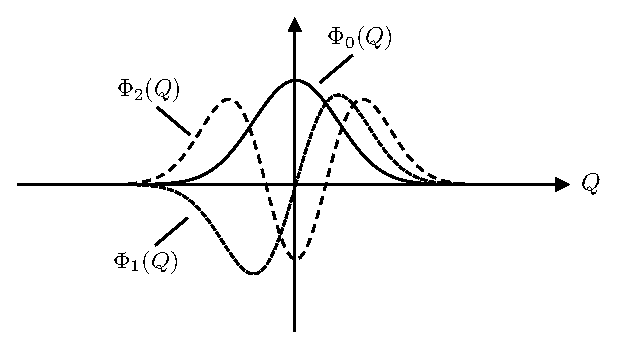
\includegraphics[width=8cm]{fig/2-2_Hermite_Gaussian.eps} 
  \caption{調和振動子のエネルギー固有状態の$Q$表示による波動関数($\Phi_0(Q), \Phi_1(Q), \Phi_2(Q)$)。}
  \label{fig:Hermite_Gaussian}
\end{figure}

\subsection{重ね合わせ状態}
前節で求めたエネルギー固有状態の波動関数は、時間とともに変化をしない解であった。ただし、シュレディンガー描像において、波動関数の位相は$\exp(-iE_kt/\hbar)$で時間とともに変化していく。

一方、式(\ref{eq:superposition_of_eigenstate})に示すように、様々な波動関数の線形結合もシュレディンガー方程式の解となる。このような複数の状態の線形結合を\textbf{重ね合わせ状態}\index{かさねあわせじょうたい@重ね合わせ状態}という。

重ね合わせ状態の例として、$\Psi(Q) = \frac 1 {\sqrt 2} (\Phi_0(Q) + \Phi_1(Q))$を考えてみよう。シュレディンガー描像では、この重ね合わせ状態は次式のように時間発展する。
\begin{equation}
  \Psi(Q, t) = \frac 1 {\sqrt 2}\left\{\Phi_0(Q)e^{-i(\omega/2) t} + \Phi_1(Q)e^{-i(3\omega/2)t}\right\} = \frac{e^{-i(\omega/2)t}}{\sqrt 2}\left\{\Phi_0(Q) + \Phi_1(Q)e^{-i\omega t}\right\}
  \label{eq:time_evolution_of_amplitude}
\end{equation}
ただし、$\Phi_0(Q)$および$\Phi_1(Q)$の固有エネルギーがそれぞれ$\hbar \omega /2$、$3\hbar \omega/2$であることを用いた。ここで、波動関数の絶対値の自乗を取り、$Q$の確率分布を求めると、次式を得る\footnote{ここでは波動関数が実数であることを用いた。波動関数の位相が位置によって異なると仮定すると、それは運動量を有していることになるので、時間とともに変化する解のはずであり、エネルギー固有状態たり得ない。したがって、エネルギー固有状態の波動関数の位相は位置によらないことから、実数で波動関数を表すことができる。}。
\begin{equation}
  \left| \Psi(Q, t)\right|^2 = \frac{1}{2}\left\{|\Phi_0(Q)|^2 + |\Phi_1(Q)|^2 + 2\Phi_0(Q)\Phi_1(Q)\cos\omega t\right\}
  \label{eq:time_evolution_of_probability}
\end{equation}
この式は以下のことを表している。図\ref{fig:Hermite_Gaussian}より、$\Phi_0(Q)$は偶関数、$\Phi_1(Q)$は奇関数であることがわかる。したがって、$\Phi_0(Q)$と$\Phi_1(Q)$を重ね合わせると、$Q>0$では強めあいの干渉、$Q < 0$では弱めあいの干渉が起こる。このため、$|\Psi(Q)|^2$は重心が$Q > 0$に偏った分布となる。この様子を図\ref{fig:superposition_state}に示す。

その後、式(\ref{eq:time_evolution_of_amplitude})で示されるように時間とともに位相が発展する。時間が$t = \pi / \omega$まで経過すると、$\Psi(Q)$は$\Phi_0(Q)$と$\Phi_1(Q)$の引き算の状態になる。このため、$|\Psi(Q)|$は重心が$Q < 0$に偏る。これを繰り返すことで、$\Psi(Q, t)$という状態は$Q$を周波数$\omega$で振動させるのである。これは、2つの波動関数のビートが生じている、と考えることができる。

次に、波動関数の位相も含めてもう少し詳しく見てみよう。時間$t = \pi/2\omega$では、式(\ref{eq:time_evolution_of_amplitude})は
\begin{equation}
  \Psi(Q) = \frac{e^{-i\pi/4}}{\sqrt 2}\left\{ \Phi_0(Q) - i \Phi_1(Q)\right\} = \frac{e^{-i\pi/4}}{\sqrt 2} \Phi_0(Q) \left\{ 1 - i\sqrt 2 Q\right\} 
\end{equation}
である。ここから$\Psi(Q)$の位相を求めると、
\begin{equation}
  \arg \Psi(Q) = -\pi/4 - \arctan \sqrt 2 Q
\end{equation}
を得る。右辺第2項から、$Q$の増加とともに位相が負に変化することがわかる。これは波数$k = \frac d {dQ} \arg \Psi(Q)$が負であることを表しており、運動量$P = \hbar k$も$-Q$の方向を向いている。同様に、時間$t = 3\pi / 2\omega$では運動量が正の値をとる。これは、図\ref{fig:classical_phase_space}(b)に示すような位相平面上の回転を表している。

ここでは$\Phi_0$と$\Phi_1$のビートで調和振動が表せることを示した。同様に考えていけば、重ね合わせの割合を変えることで振動振幅を変えることができることもわかるであろう。実際、たくさんの解を用いて重ね合わせの係数をうまく設定することで、様々な振幅の調和振動を表すことができる。これはコヒーレント状態と呼ばれるものであり、次章で説明する。

\begin{figure}
  \centering
  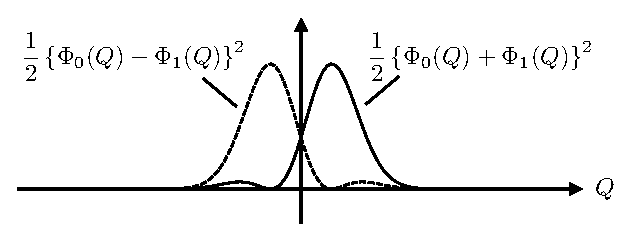
\includegraphics[width=8cm]{fig/2-3_superposition_state.eps} 
  \caption{重ね合わせ状態の波動関数の絶対値の自乗。$Q$の確率分布が重ね合わせの符号によって変化することがわかる。}
  \label{fig:superposition_state}
\end{figure}

\begin{comment}
$p, q$に対しては、
\begin{equation}
  \braket{\Delta \hat q^2}\braket{\Delta \hat p^2}\geq \frac{\hbar^2}{4}
\end{equation}
\begin{equation}
  \braket{\Delta \hat Q^2}\braket{\Delta \hat P^2}\geq \frac{1}{4}
\end{equation}
が成り立つ。
\end{comment}

\section{まとめ}
本章では以下の事柄について説明を行った。
\begin{itemize}
	\item シュレディンガー描像とシュレディンガー方程式。シュレディンガー描像では状態ベクトルが時間発展する。その時間発展を記述する方程式がシュレディンガー方程式である。また、時間発展に伴う状態ベクトルの変化は時間発展演算子で記述できる。
	\item ハイゼンベルグ描像とハイゼンベルグの運動方程式。ハイゼンベルグ描像では物理量の演算子を変化させることで時間発展を考える。このときの演算子の変化を記述するのがハイゼンベルグの運動方程式である。
	\item 調和振動子のハミルトニアンは位置エネルギーと運動エネルギーの和になる。
	\item 調和振動子のエネルギー固有状態は非負の整数$n$を用いて$\ket n$で表される。量子光学ではこの$n$を光子数に対応させる。
	\item 生成・消滅演算子。エネルギー固有状態をひとつづつ変化させる役割を持つ。同時に、消滅演算子は複素振幅の演算子でもある。
\end{itemize}
また、本節で説明した演算子について、表\ref{table:operator_of_quantity}にまとめた。これらは次章以降で頻繁に現れることになる。


\begin{table}
\caption{物理量の演算子とその意味}	
\begin{center}
\begin{tabular}{c c}
\hline
	演算子 & 意味 \\
	\hline \hline
	$\hat Q$ & 規格化された位置\\
	$\hat P$ & 規格化された運動量\\
	$\hat a$ & 複素振幅(エルミートではないので注意)\\
	$\hat a ^\dagger \hat a = \hat n$ & 量子数もしくは光子数\\
	$\hat a_1 = (\hat a + \hat a^\dagger)/2 = \hat Q/\sqrt 2$ & 複素振幅の実部\\
	$\hat a_2 = (\hat a - \hat a^\dagger)/2i = \hat P/\sqrt 2$ & 複素振幅の虚部\\
\hline
\end{tabular}
\label{table:operator_of_quantity}
\end{center}
\end{table}



\chapter{光の量子状態}

本章では、まず、光を調和振動子の集まりとして考える手続きについて述べる。その後、代表的な光の量子状態である、光子数状態、コヒーレント状態、スクイズド状態を説明する。特に、これらが複素振幅や光子数についてどのような揺らぎを有するのかを説明する。

\section{量子光学の手続き}
量子光学では、以下のような手続きで、光を調和振動子に対応させる。

まず、光を色々な空間モード、周波数モード、偏光に分解する。その分解の仕方に関してはひとつに決まっているわけではない\footnote{その理屈は、正規直交基底の取り方が複数あるのと同じである。分解の仕方によって計算結果が変わってくるわけではない。}。

例えば、レーザからビーム状の光が出力されている状況を考えよう。このレーザビームの空間分布は非常に安定している、すなわち横モードがシングルモードであるとし、また、偏光は単一であるとする。このビームが進む方向を$z$方向とし、時間$-\Delta t/2 \leq t < \Delta t/2$において$z = 0$を通過する光について考えるものとする。

この時間における光電界の時間波形を$s(t)$とし、$s(t)$のフーリエ変換$S(\omega)$を考えよう。以下のように$S(\omega)$は角周波数$\Delta \omega = 2\pi / \Delta t$間隔のスペクトルからなることがわかる\footnote{ここに書いてあることは、要は「各空間モード・周波数モードは複数の基底の線型結合で表現できて、全ての基底に対する複素振幅を決めれば元の波形を表現できるよ」ということだけであるので読み飛ばしても構わない。なお、このときの基底の数のことを「自由度」という。}。

まず、$s(t)$を周期関数化した$s_1(t) = \sum_{m = -\infty}^{\infty}s(t-m\Delta t)$を考える。$s_1(t)$のフーリエ変換$S_1(\omega)$は周期関数のフーリエ変換であるから、
角周波数$\Delta \omega = 2\pi/\Delta t$の離散スペクトルから構成される。ここで、$s(t) = s_1(t)\mathrm{rect}(t / \Delta t)$である\footnote{$\mathrm{rect}(t)$は$(|t|<1/2)$の時1、それ以外で0を取る関数である。}から、$S(\omega)$は、$S_1(\omega)$に$\mathrm{rect}$関数のフーリエ変換である$\mathrm {sinc}$関数を畳み込んだものである。このように考えると、$S(\omega)$の自由度は、離散スペクトルの自由度と等しく、周波数帯域を$\Omega$とすれば、$\Omega/\Delta\omega$個の複素数(フーリエ係数)で$s(t)$を表すことができる。

このとき、$\Delta t$の値を2倍にすると、離散スペクトルの周波数間隔$\Delta \omega$が半分になるので、自由度の数は2倍になる。これは、計測時間$\Delta t$を保ったまま、2回計測を行ったときの自由度の数と同じである。このことから想像できるように、時間波形をフーリエ変換してスペクトル分解する際は、$\Delta t$の切り方をどのようにしても良い。時間幅$\Delta t$と周波数帯域$\Omega$が決まれば、その自由度は$\Omega\Delta t/2\pi$個となる。

実際には、$\Delta t$は考えやすい値に設定することが多い。例えば、光ファイバ通信においては1ビットの光に1つの自由度を設定したり、光パルスであれば1つの光パルスに1つの自由度を設定する等である。もちろん、1つの光パルスの中で強度や位相が変化する場合などは、複数の自由度を考える必要がある。いずれにせよ、このようにして、時間・周波数領域で複数の自由度に分解することができる。

光の周波数が決まれば、複数の空間モードに展開することができる。その展開の仕方も、正弦波(平面波)で展開する方法、エルミートガウスモードで展開する方法など様々な方法が考えられる。ただ、ここでは簡単のため、空間モードは単一であるとしよう。シングルモード光ファイバー中の光や、単一横モードのレーザーの出力を考えるときにはこれで十分である。

一旦、このようにモードに分解できたら、その単一のモードに注目する。時間$\Delta t$の間に光が進む距離は$L = c\Delta t/n$であるから、その間の光が持つエネルギーは、
\begin{equation}
U = \frac 1 2 \int_V \left(\varepsilon E^2 + \mu H^2\right)dr = \int_V \varepsilon E^2 dr
\end{equation}
と求められる。ここで、$\frac 1 2 \varepsilon E^2$は電界が有する単位体積あたりのエネルギー、$\frac 1 2 \mu H^2$は磁界が有する単位体積あたりのエネルギーであり、電界と磁界のエネルギーが等しいことを用いた。また、$V$は空間モードの体積である。

%\textbf{この辺り怪しい。式(3.3)は教科書通りだが。。。$p^2/2$は運動エネルギーで、その時間平均は$p^2/4$となる。$(1/2)\varepsilon E^2$は電場のエネルギーで、それを空間$V$で平均すると$(1/4)\varepsilon V E^2$になる。磁場のエネルギーはこれと同じ。$p^2/4$と$(1/4)\varepsilon V E^2$}

%単純に、$(1/2)\varepsilon VE^2$を$(1/2)p^2$に対応させれば良いはず。

量子光学では、このひとつのモードを、同じエネルギーを有する調和振動子に対応させる。慣例的に、$E \propto -p$となるようにすることが多い
\footnote{これは、場の量子論においてベクトルポテンシャル$\pmb A$の一つのモードを調和振動子の位置$q$に対応させるためである。理論的には、電界$E$を$q$に対応させても$p$に対応させても、調和振動子の位相が異なるだけなので何の問題も生じないが、ここでは物理系の流儀に合わせてこのような定義を採用する。}。
$E$の振幅が空間的に一様であるとすれば、$U = \frac 1 2 \varepsilon V E^2$であり、これが運動エネルギー$\frac 1 2 p^2$と一致するようにするため、$t = 0$、$z = 0$において
\begin{equation}
  E = -\frac 1 {\sqrt {\varepsilon V}}p
\end{equation}
とおく。ここで、$E$と$p$を演算子で表すと、次式を得る。
\begin{equation}
  \hat E = -\frac 1 {\sqrt{\varepsilon V}}\hat p = i\sqrt{\frac{\hbar \omega}{2\varepsilon V}}(\hat a - \hat a^\dagger)
\end{equation}
$\hat E$の$t$および$z$の依存性は、演算子をハイゼンベルグ描像で時間発展及び空間発展させることで次式のように表せる。
\begin{equation}
  \hat E(x,y,z,t) = i\sqrt{\frac{\hbar \omega}{2\varepsilon V}}(\hat a e^{i(kz-\omega t)} - \hat a^\dagger e^{-i(kz-\omega t)})
\end{equation}

なお、この式は、電場が空間的に一様であるという仮定を置いた近似式である。本来は、ビームの空間分布を考え、位置によって電場の大きさや位相が異なることを表さなければならない。とはいえ、そのような取り扱いをしたとしても、ひとつの空間モードを調和振動子として表すことに変わりないので、ここではこれ以上深入りしない。

各モードを調和振動子に対応させられることがわかったので、次は、光(量子的調和振動子の)の代表的な量子状態である、光子数状態、コヒーレント状態、スクイズド状態について説明する。これらの量子状態は、対応する状態ベクトル$\ket \phi$で表される。

$\ket \phi$の性質を知るには、この状態に対して物理量の計測を行った時の期待値を計算していけば良い。前章で述べたように、物理量$\hat A$と状態ベクトル$\ket \phi$が決まれば、物理量の期待値を計算することができる。ここで用いる物理量としては、光子数$\hat n = \hat a^\dagger \hat a$, $\hat a$の実部$\hat a_1 = \frac{1}{2}(\hat a + \hat a^\dagger) = \frac{1}{\sqrt 2}\hat Q$, および$\hat a$の虚部$\hat a_2 = \frac{1}{2i}(\hat a - \hat a^\dagger$)等がある。


\section{光子数状態}

$\ket \phi$が$\ket 0, \ket 1, \ket 2, \ket 3, \hdots$のいずれかである時、これは光子数が一意に決まった状態であるから、光子数状態という。光子数状態$\ket n$に対する光子数の期待値は、
\begin{equation}
  \braket{n|\hat a^\dagger \hat a|n} = n\braket{n|n} = n
\end{equation}
である。また、光子数の分散は、
\begin{equation}
\braket{n|(\hat a^\dagger \hat a)^2|n} - n^2 = n\braket{n|\hat a^\dagger \hat a|n} - n^2 = n^2 - n^2 = 0  
\end{equation}
となる。このように、光子数状態では光子数が確定しており、そのゆらぎはない。

次に、実部$\hat a_1$を見てみよう。その期待値は、
\begin{equation}
\begin{aligned}
  \braket{n|\hat a_1|n} &= \braket{n|\frac{\hat a + \hat a^\dagger}{2}|n} = \frac 1 2 \braket{n|\hat a|n} + \frac{1}{2}\braket{n|\hat a^\dagger|n}\\
  &= \frac{\sqrt n}{2}\braket{n|n-1} + \frac{\sqrt{n + 1}}{2}\braket{n|n+1} = 0
\end{aligned}
\end{equation}
であり、また、分散は、平均が0であることから2乗の平均と等しく、
\begin{equation}
\begin{aligned}
  \braket{n|\hat a_1^2|n} &= \frac{1}{4}\braket{n|\hat a\hat a+\hat a \hat a^\dagger + \hat a^\dagger \hat a + \hat a^\dagger \hat a^\dagger|n} \\
  &= \frac{1}{4}\braket{n|\hat a \hat a^\dagger + \hat a^\dagger \hat a|n}\\
  &= \frac{1}{4}\braket{n|2\hat a^\dagger \hat a + 1|n} = \frac{1}{2}\left(n + \frac 1 2\right)  
  \label{eq:variance_Fock_real}
\end{aligned}
\end{equation}
を得る。同様に、虚部$\hat a_2$に対しても、
\begin{equation}
  \braket{n|\hat a_2|n} = 0
\end{equation}
\begin{equation}
  \braket{n|\hat a_2^2|n} = \frac{1}{2}\left(n + \frac 1 2\right)
  \label{eq:variance_Fock_imag}
\end{equation}
が成り立つ。

式(\ref{eq:variance_Fock_real})(\ref{eq:variance_Fock_imag})は、$n = 0$においても、複素振幅の実部、虚部がゆらぎを持つことを表している。このゆらぎのことを\textbf{真空場ゆらぎ}という。
真空場は、図\ref{fig:vacuum_field}に示すイメージ図のように、複素振幅の実部・虚部に1/4の分散を有する。この2つの分散の和が1/2であることは、基底状態$\ket 0$のエネルギーが$\frac 1 2 \hbar \omega$であることと対応している。
%\footnote{$\ket 1, \ket 2, \hdots$が複素平面上でどのような分布を取るかは付録に示す。}

\begin{figure}
  \centering
  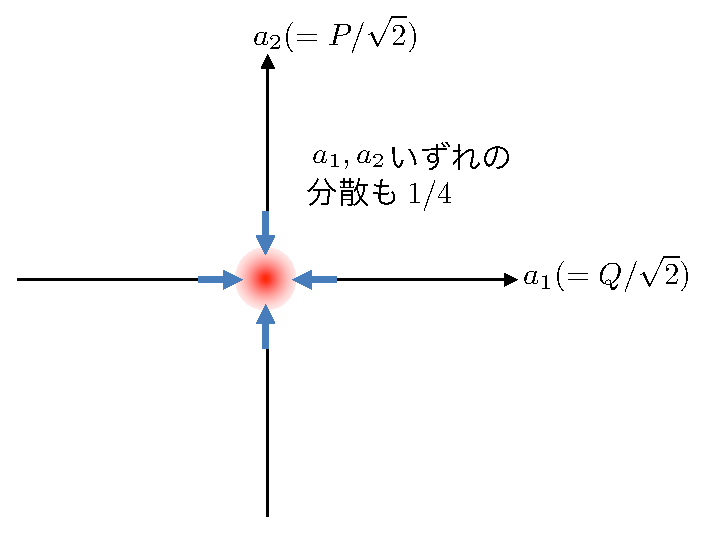
\includegraphics[width=8cm]{fig/3-1_vacuum.eps} 
  \caption{真空場の複素振幅のイメージ。}
  \label{fig:vacuum_field}
\end{figure}

また、光子数状態は光の波動としての位相の情報を持たない。古典的な波動は、周波数$\omega$で時間変化し、その変化のタイミングが位相に対応する。一方、光子数状態はハミルトニアン(時間発展演算子)の固有状態であり、時間とともに変化をしない状態である。ただ、計測される光子数は一意に決まり、計測される複素振幅にはゆらぎがある。

なお、厳密な光子数状態を作るのは技術的に大変難しいが、最近では量子ドット等を用いて光子数状態を発生させることができつつあり、量子暗号等への応用が期待されている。

また、光子数状態は正規直交系であり、光子数状態以外の量子状態は、複数の光子数状態の重ね合わせとして表される。これが、検出される光子数のばらつきに対応する。


\begin{comment}
\subsubsection{光子数状態の重ね合わせ}
光子数状態は時間とともに変化しない状況であった。一方、異なる光子数状態を重ね合わせると、時間とともに変化する量子状態を作ることができる。

例として、$\ket \phi = \frac{1}{\sqrt 2}(\ket 0 + \ket 1)$を考えてみよう\footnote{$\frac{1}{\sqrt 2}$のファクタは、規格化($\braket{\phi|\phi} = 1$)のためにつけた。}。シュレディンガー描像では、エネルギー$E_n = \frac{1}{2}(n + 1/2)$を有するエネルギー固有状態は角周波数$\omega_n = E_n / \hbar = \omega (n + \frac 1 2)$で時間発展する。また、したがって、
\begin{equation}
\begin{aligned}
  \ket {\phi (t)} &= \frac 1 {\sqrt 2}\left(\ket 0 e^{-i\omega (1/2)} + \ket 1 e^{-i\omega (1 + 1/2)}\right)\\
  &= \frac{e^{-i\omega t/2}}{\sqrt 2}\left( \ket 0 + \ket 1 e^{-i\omega t}\right)
\end{aligned}
\end{equation}
を得る。$t = 0$では$\ket{\phi(0)} \propto {\ket 0 + \ket 1}$, $t = \pi/\omega$では$\ket{\phi(\pi/\omega)} \propto {\ket 0 - \ket 1}$となり、時間発展とともにこれを繰り返すことがわかる。
$\ket 0$、$\ket 1$の$Q$表示(図?)を考えると、$\ket 0 = \ket 1$は、波動関数の分布が$+Q$の方向に偏っている一方、$\ket 0 - \ket 1$は$-Q$の方向に偏っている。このように、異なる光子数状態を重ね合わせることで、周波数$\omega$で振動する光を表すことができる。
\end{comment}

\section{コヒーレント状態}
複数の光子数状態の重ね合わせとして次式で表される状態を\textbf{コヒーレント状態}という。
\begin{equation}
  \ket \alpha = \exp \left( -\frac{|\alpha|^2}{2} \right)\sum_{n = 0}^{\infty}\frac{\alpha^n}{\sqrt{n!}} \ket n
  \label{eq:coherent_state}
\end{equation}
コヒーレント状態はレーザーでつくられる正弦波的な波動に対応する量子状態であり、複素振幅$\alpha$を有し、また、振幅及び光子数のゆらぎを有する。

式(\ref{eq:coherent_state})の右辺のうち、コヒーレント状態の性質を決める重要な項は$\ket n$の線形結合を取っている部分である。一方、$\exp$の部分は、$\braket {\alpha|\alpha} = 1$とするための規格化因子である。

以下では、コヒーレント状態が持つ幾つかの性質を見ていこう。

\subsection{消滅演算子の固有状態}
$\ket \alpha$は、消滅演算子$\hat a$の固有状態であることが知られている。このことは以下のように示される。
\begin{equation}
\begin{aligned}
	  \hat a \ket \alpha &= \exp\left(-\frac{|\alpha|^2}{2}\right)\sum_{n = 0}^\infty \frac{\alpha^n}{\sqrt{n!}}\sqrt n \ket{n - 1}\\
	  &=\alpha \exp\left(-\frac{|\alpha|^2}{2}\right)\sum_{n = 1}^\infty\frac{\alpha^{n - 1}}{\sqrt{(n - 1)!}}\ket{n - 1}\\
	  &=\alpha \ket \alpha
\end{aligned}
\end{equation}
なお、2行目で和が$n = 1$から始まっているのは、$\hat a\ket 0 = 0$であることを利用したためである。
また、このエルミート共役を取ると、$\bra \alpha \hat a^\dagger = \alpha^* \bra \alpha$である。

なお、$\hat a$がエルミート演算子でない($\hat a^\dagger \neq \hat a$)ことに注意が必要である。このため、$\ket \alpha$は$\hat a$の固有状態ではあるが、$\alpha$を誤差なく直接測定することはできない。また、固有状態$\ket \alpha$は正規直交基底にはなっていない。これらの性質は後に述べる。

\subsection{光子数の分布}
コヒーレント状態で$n$個の光子を検出する確率を$P(n)$とする。$P(n)$を求めるには、光子数状態$\ket n$との内積を取り、そのノルムを求めればよいから、次式のように計算できる。
\begin{equation}
\begin{aligned}
  P(n) &= |\braket {n | \alpha}|^2 = \left| \exp\left(-\frac{|\alpha|^2}{2}\right) \frac{\alpha^n}{\sqrt{n!}}\right|^2\\
  &= \exp \left(-|\alpha|^{2}\right)\frac{|\alpha|^{2n}}{n!}\\
  &\equiv \exp \left(-\lambda\right)\frac{\lambda^n}{n!}
\end{aligned}
\end{equation}
ただし、3行目で$\lambda = |\alpha|^2$とおいた。このように、コヒーレント状態の光子数の分布はポアソン分布となる。

コヒーレント状態は、光が波動でありながらも、光子が確率的に到来し、ショット雑音を生むことを表している。

\subsection{複素振幅の期待値と分散}
複素振幅の演算子である$\hat a$はエルミートでないのでその測定を行うことはできない。しかし、複素振幅の実部を
\begin{equation}
  \hat a_1 = \frac 1 2 (\hat a + \hat a^\dagger)
\end{equation}
と定義すれば、$\hat a_1^\dagger = \hat a_1$より$\hat a_1$はエルミートであるから、その測定を行うことができる。同様に、複素振幅の虚部を
\begin{equation}
  \hat a_2 = \frac 1 {2i} (\hat a - \hat a^\dagger)
\end{equation}
と定義すれば、$\hat a_2$も同様にエルミートとなり、その測定が可能である。

コヒーレント状態$\alpha$に対して、複素振幅の実部$\hat a_1$の期待値と分散を求めよう。なお、ここでは$\braket{\alpha|\hat a_1|\alpha} \equiv \braket{\hat a_1}$のように表すこととする。
\begin{equation}
\begin{aligned}
  \braket{\hat a_1} &= \frac{1}{2}\braket{\alpha|\hat a + \hat a^\dagger|\alpha} = \frac{1}{2}\braket{\alpha|\hat a |\alpha} + \frac{1}{2}\braket{\alpha|\hat a^\dagger |\alpha}\\
  &= \frac{1}{2}\alpha \braket{\alpha|\alpha} + \frac{1}{2} \alpha^* \braket{\alpha|\alpha} = \frac 1 2 (\alpha + \alpha^*) = \mathrm{Re} \ \alpha
\end{aligned}
\end{equation}

\begin{equation}
\begin{aligned}
  \braket{\hat a_1^2} &= \frac{1}{4}\braket{\alpha|(\hat a + \hat a^\dagger)^2|\alpha} = \frac{1}{4}\braket{\alpha|\hat a \hat a + \hat a \hat a^\dagger + \hat a^\dagger \hat a + \hat a^\dagger \hat a^\dagger|\alpha}\\
  &= \frac 1 4 \braket{\alpha|\hat a \hat a + 2\hat a^\dagger \hat a + 1 + \hat a^\dagger \hat a^\dagger|\alpha}\\
  &= \frac{1}{4}\left\{\alpha^2 + 2|\alpha |^2 + 1 + (\alpha^*)^2\right\}
\end{aligned}
\end{equation}
\begin{equation}
	\begin{aligned}
		\braket{\hat a_1^2} - \braket{\hat a _1}^2 &= \frac{1}{4}\left\{\alpha^2 + 2|\alpha |^2 + 1 + (\alpha^*)^2\right\} - \frac{1}{4}\left\{\alpha^2 + \alpha \alpha^* + \alpha^*\alpha + (\alpha^*)^2\right\} = \frac 1 4
	\end{aligned}
\end{equation}
したがって、コヒーレント状態$\ket \alpha$の複素振幅の実部$\hat a_1$を計測すると、その平均値は$\mathrm {Re} \ \alpha$、分散が$\frac 1 4$であることがわかる。

同様に、虚部$\hat a_2$を計測すると、その平均値は$\mathrm{Im} \ \alpha$、分散が$\frac 1 4$であることを示すことができる。この分散は真空状態$\ket 0$の分散と同じである。

この様子を元に、$\ket \alpha$を複素平面のように表したものを図\ref{fig:coherent_state}に示す。$(\mathrm {Re} \ \alpha, \mathrm{Im} \ \alpha)$を中心として、実部、虚部にいずれも1/4の分散を有するように描いている。このように、広がりのある複素振幅が、時間発展とともに$e^{-i\omega t}$のように回転していく。実部に注目すると、広がりを持ったまま正弦波で振動しており、虚部に注目しても同様である。このように、コヒーレント状態は、調和振動子の複素振幅が広がりを持ったまま時間発展する様子と考えることができる。

一方、このような図を解釈するときには注意が必要である。なぜなら、$\hat a_1$と$\hat a_2$は同時に測定できないためである。($[\hat a_1, \hat a_2] = i/2$である。)
\begin{figure}
  \centering
  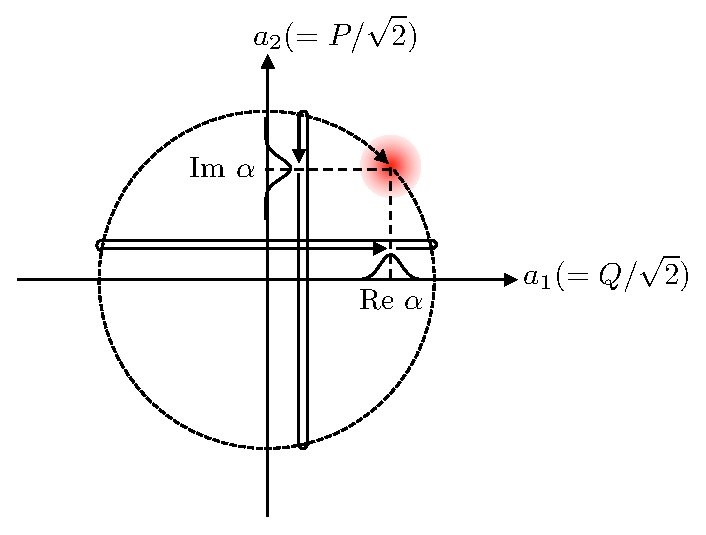
\includegraphics[width=8cm]{fig/3-2_coherent_state.eps} 
  \caption{コヒーレント状態の複素振幅のイメージ。複素振幅の実部$a_1$の中心はRe $\alpha$、虚部$a_2$の中心はIm $\alpha$にあり、その分散は真空場と同じ1/4である。シュレディンガー描像で時間発展すると、$a_1$の分布と$a_2$の分布のいずれも正弦波状に振動する。このとき、$a_1$と$a_2$の分布($\hat a_1$と$\hat a_2$は同時に計測できないことに注意)は、$a_1-a_2$平面上で回転する。}
  \label{fig:coherent_state}
\end{figure}

\subsection{変位演算子によるコヒーレント状態の生成}
前節で見たように、コヒーレント状態は、その複素振幅の分散が真空場$\ket 0$と同じであり、複素振幅が$\alpha$であるような状態である。このことに注目すると、$\ket 0$に対して複素振幅を少しずつ変化させていく操作を加えると、コヒーレント状態を生成することができる。

このように、複素振幅を変化させる演算子を変位演算子といい、次式で与えられる。
\begin{equation}
  \hat D(\alpha) = \exp(\alpha \hat a^\dagger - \alpha^*\hat a)
\end{equation}
変位演算子はユニタリ演算子であり、これを用いて、
\begin{equation}
  \ket \alpha = \hat D(\alpha)\ket 0
\end{equation}
であることを示すことができる。この証明には、Baker-Cambell-Hausdorffの公式と呼ばれるものを用いる。これは、$[\hat A, [\hat A, \hat B]] = [\hat B, [\hat A, \hat B]] = 0$のとき、$\exp(\hat A + \hat B) = \exp \hat A \exp \hat B \exp \left(-\frac{1}{2} [\hat A, \hat B]\right)$が成り立つ、というものであり、これに$\hat A = \alpha \hat a^\dagger$、$\hat B = -\alpha^*\hat a$とすれば左辺は$\hat D(a)$となる。ここで$\hat D(\alpha) \ket 0$を計算すると、式(\ref{eq:coherent_state})を得る。

とはいえ、この証明はあまり直感的でないので、ここでは少し違う観点から変位演算子の働きを調べておこう。演算子$\hat H = i\hbar(\alpha\hat a^\dagger - \alpha ^*\hat a)$を考えると、これは$\hat H^\dagger = \hat H$であることから、エルミートであることがわかる。これをハミルトニアンとする時間発展演算子を考える\footnote{ここでの$t$はもはや時間ではなく、ケットベクトルを徐々に変化させるためのパラメータである。}と、
\begin{equation}
\hat U(t) = \exp\left(\frac{t}{i\hbar}\hat H\right) = \exp\left\{t(\alpha\hat a^\dagger - \alpha^* \hat a)\right\}
\end{equation}
であるから、$\hat U(1) = \hat D(\alpha)$である。
ここで、$t = 0 \to 1$で$\hat a$, $\hat a^\dagger$が$\hat a'$, $\hat a'^\dagger$に変化すると考えよう。ハイゼンベルグの運動方程式から、
\begin{equation}
 \frac{d}{dt}\hat a = \frac i \hbar[\hat H, \hat a] = -\alpha [\hat a^\dagger, \hat a] = \alpha
\end{equation}
\begin{equation}
  \frac{d}{dt}\hat a^\dagger = \frac i \hbar [\hat H, \hat a^\dagger] = \alpha^*[\hat a, \hat a^\dagger] = \alpha^*
\end{equation}
したがって、
\begin{equation}
  \hat a' = \hat a + \alpha
\end{equation}
\begin{equation}
  \hat a'^\dagger = \hat a^\dagger + \alpha ^*
\end{equation}
である。これは、ある状態ベクトルに変位演算子$\hat D(\alpha)$を作用させると、複素振幅が$\alpha$だけ変化することを表している。

\subsection{ショット雑音と真空場}
コヒーレント状態は直感的に「複素振幅$\alpha$の周りに真空場があるもの」と捉えることができる。コヒーレント状態の平均の光子数は
\begin{equation}
  \braket{\hat n} = \braket{\alpha | \hat n |\alpha} = \braket {\alpha |\hat a^\dagger \hat a|\alpha} = |\alpha|^2
\end{equation}
である。したがって、
\begin{equation}
  |\alpha| = \sqrt{\braket {\hat n}}
\end{equation}
である。また、コヒーレント状態において複素振幅の実部・虚部のいずれも1/4の分散を有しており、その標準偏差は$\sqrt{1/4} = 1/2$である。このことから、$|\alpha|$の標準偏差も1/2である\footnote{半径方向の標準偏差が実部の標準偏差と等しいことは、コヒーレント状態を時間発展させて複素振幅が実数になった瞬間の広がりを考えると理解できる。}。

このことから、複素振幅の半径方向の揺らぎによって、光子数がどれだけ変化するかを計算すると、
\begin{equation}
  \left\{\sqrt n \pm \frac 1 2\right\}^2 = n \pm \sqrt n + 1/4
\end{equation}
を得る。$\pm \sqrt n$は、光子数の揺らぎ、すなわちショット雑音を表している。このように、揺らぎのない正弦波に、真空場の揺らぎを足し合わせて、その絶対値の自乗を取ることで強度の揺らぎが現れたものとして、ショット雑音を捉えることができる。言い換えると、ショット雑音は、正弦波と真空場とのビートである、と考えると良い。



\subsection{コヒーレント状態と光損失}
コヒーレント状態の光が、光損失を受けて強度が減少した状況を考えよう。この光も、コヒーレント状態となることが知られている。このことは次章で示そう。

損失を受けて複素振幅が小さくなっても、真空場揺らぎは変化しないので、損失によって、光の信号対雑音比が減少することがわかる。

\subsection{コヒーレント状態の非直交性}
先述のように、コヒーレント状態$\ket \alpha$は、非エルミート演算子である$\hat a$の固有状態であるため、必ずしも正規直交系を作らない。実際、複素振幅$\alpha, \alpha'$を有するコヒーレント状態$\ket \alpha, \ket \alpha'$の内積を計算すると、次式を得る。
\begin{equation}
\begin{aligned}
  \left| \braket{\alpha'|\alpha}\right|^2 &= \left| \exp\left(-\frac{|\alpha'|^2}{2}\right)\exp\left(-\frac{|\alpha|^2}{2}\right)\sum_{n = 0}^\infty \frac{\left(\alpha'^*\alpha\right)^n}{n!} \right|^2\\
  &=\exp(-|\alpha'|^2 - |\alpha|^2)\left|
  \sum_{n=0}^\infty \frac{\left(\alpha'^*\alpha\right)^n}{n!}
  \right|^2\\
  &=\exp(-|\alpha'|^2 - |\alpha|^2)\left|\exp(\alpha'^*\alpha)
  \right|^2\\
  &= \exp(-|\alpha'|^2 - |\alpha|^2 + \alpha'^*\alpha +\alpha'\alpha^*)\\
  &= \exp(-|\alpha' - \alpha|^2)
\end{aligned}
\end{equation}
したがって、$|\alpha' - \alpha|$が大きいほど内積が小さくなり、0に収束する。しかし、どれだけ離れても0になることはない。このことから、コヒーレント状態は直交基底とはなっていない。
\begin{comment}
\subsection{光子数状態とコヒーレント状態の関係}


スペクトログラムで書くと時間発展は回転で表される。

\begin{equation}
  \braket{\alpha|n} = \bra{\alpha}\frac{(\hat a^\dagger)^n}{\sqrt{n!}}\ket 0 = \frac{(\alpha^*)^n}{\sqrt {n!}} \braket{\alpha|0} = \frac{(\alpha^*)^n}{\sqrt {n!}} \exp(-|\alpha|^2)
\end{equation}

\begin{equation}
  \braket{\alpha|\phi} = \sum_k c_k\braket{\alpha|k} = \sum_k \frac{c_k}{\sqrt{k!}}(\alpha^*)^k \exp(-|\alpha|^2)
\end{equation}

\begin{equation}
  \hat a_1 \ket n = \frac{1}{2}(\hat a + \hat a^\dagger)\ket n = 
\end{equation}

\end{comment}


\section{スクイズド状態}
コヒーレント状態は、複素振幅の実部と虚部に等しい揺らぎを持つ状態であった。一方、例えば虚部が大きな揺らぎを持つことを許せば、実部の揺らぎを小さくすることが可能である\footnote{複素振幅の実部$a_1$と虚部$a_2$の波動関数は互いにフーリエ変換の関係にある。これは位置$Q$と運動量$P$の波動関数がフーリエ変換の関係にあることと同様である。このように考えると、実部の波動関数の幅を狭めると、虚部の波動関数の揺らぎが大きくなることは想像しやすい}。このようにして複素振幅のある方向の揺らぎを小さくした光の量子状態のことを、スクイズド状態\footnote{厳密にはこれ以外のスクイズド状態もある。複素振幅の実部と虚部の揺らぎの配分を変えた状態を直交スクイズド状態という。}という。

スクイズド状態は光パラメトリック増幅と呼ばれる技術を用いて発生することが可能である。その詳細は非線形光学の章で扱う。

スクイズド状態の技術的な困難性は、光の損失に弱い点にある。スクイズド状態の光に対して光損失が生じると、コヒーレント状態に近づいていき、スクイーズの度合いが弱まってしまう。
\subsection{スクイズド状態}

コヒーレント状態$\ket \alpha$からスクイズド状態$\ket \beta$に変換するユニタリ演算子を$\hat S(r)$としよう。すなわち、
\begin{equation}
  \ket \beta = \hat S(r) \ket \alpha
\end{equation}
とすると、
\begin{equation}
  \hat S(r)=\exp\left[\frac r 2 \{\hat a^2 - (\hat a^\dagger)^2\}\right]
\end{equation}
であることが知られている。$\hat S(r)$は、ハミルトニアン
\begin{equation}
	\hat H = \frac{i\hbar}{2}\{\hat a^2 - (\hat a^\dagger)^2\}  
	\label{eq:squeezing_hamiltonian}
\end{equation}
に対する時間発展演算子$\exp\left(\frac{r}{i\hbar}\hat H\right)$と捉えることができる。

このハミルトニアンを使って、ハイゼンベルグ描像で消滅演算子がどのように変化するかを見てみよう。スクイージング後の消滅演算子を$\hat b = \hat S^\dagger(r)\hat a\hat S(r) \equiv \hat a(r)$
とすると、次式が成り立つ。
\begin{equation}
  	\frac{d}{dr}\hat a = \frac{i}{\hbar}[\hat H, \hat a] = -\hat a^\dagger\\
\end{equation}
\begin{equation}
    	\frac{d}{dr}\hat a^\dagger = \frac{i}{\hbar}[\hat H, \hat a^\dagger] = -\hat a
\end{equation}
これらを用いると、
\begin{equation}
  \frac{d}{dr}\hat a_1 = \frac{d}{dr} \left(\frac {\hat a + \hat a^\dagger}{2}\right) = -\frac {\hat a^\dagger + \hat a}{2} = -\hat a_1
\end{equation}
\begin{equation}
  \frac{d}{dr}\hat a_2 = \frac{d}{dr} \left(\frac {\hat a - \hat a^\dagger}{2i}\right) = \frac {-\hat a^\dagger + \hat a}{2i}= \hat a_2
\end{equation}
であるから、
\begin{equation}
  \hat b_1 = \hat a_1(r) = \hat a_1(0) e^{-r}
\end{equation}
\begin{equation}
  \hat b_2 = \hat a_2(r) = \hat a_2(0) e^r
\end{equation}
である。このことから、
%図?に示すように、
$\hat b$の実部の分布は$e^{-r}$倍に縮小され、$\hat b$の虚部の分布は$e^{r}$倍に拡大される。

最終的に次式を得る。
\begin{equation}
\begin{aligned}
  \hat b &= \hat b_1 + i\hat b_2 = \hat a_1 e^{-r} + i\hat a_2 e^r \\
  &= \frac{1}{2} (\hat a + \hat a^\dagger)e^{-r} + \frac{i}{2i}(\hat a - \hat a^\dagger)e^{r}\\
  &= \hat a \cosh r - \hat a^\dagger \sinh r 
\end{aligned}
\end{equation}

この$\hat b$の固有状態を$\ket {\beta'}$とすると、$\ket {\beta'} = \hat S^\dagger(r)\ket \alpha$、すなわち逆スクイーズされた状態(実部が引き伸ばされ、虚部が縮んだ状態)である。また、その固有値は$\alpha$である。このことは以下のように示される。
\begin{equation}
\begin{aligned}
  \hat b\ket {\beta'} &= \hat S^\dagger(r)\hat a \hat S(r) \hat S^\dagger \ket \alpha \\
  &= \hat S^\dagger \hat a \ket \alpha \\
  &= \alpha \hat S^\dagger(r)\ket \alpha = \alpha \ket{\beta'}
\end{aligned}
\end{equation}


\subsection{スクイーズされた真空}
光子数0の状態、すなわち$\ket 0$は真空状態とも呼ばれ、複素振幅の実部・虚部に等しい揺らぎを有する。真空状態にスクイーズ演算子$\hat S(r)$を作用させると、複素振幅の平均は0でありながら、実部・虚部の揺らぎの分布を変化させることができる。このことを、\textbf{スクイーズされた真空状態}という。

スクイーズのハミルトニアン(式(\ref{eq:squeezing_hamiltonian}))を見ると、光子を2個作る演算子$(\hat a^\dagger)^2$と光子を2個減らす演算子$\hat a^2$からできていることが見て取れる。一方、真空の光子数は0である。従って、スクイーズされた真空は偶数個の光子数状態の線形結合で表されることがわかる。

直感的には、光子数状態の$Q$表示において、$\frac{1}{\sqrt 2}(\ket 0 - \ket 2)$を考えると、$Q$の分布が狭くなることが想像しやすい。これをすべての偶数個の光子数状態を適切な割合で重ね合わせると、$Q$表示において幅の狭い分布を作ることができる\footnote{このことは次のように考えることもできる。光子数状態は正規直交系であるから、$Q$表示において、任意の分布を光子数状態で展開する際は、光子数状態との内積を取れば良い。偶数個、奇数個の光子数状態の$Q$表示はそれぞれ偶関数、奇関数になっている。一方、スクイーズされた真空状態は原点に対して偶関数である。このことからも、スクイーズされた真空状態が偶数個の光子数状態の和であることがわかる。}。$P$表示は$Q$表示のフーリエ変換であるから、$Q$表示で幅の狭い分布は、$P$表示において幅の広い分布になる。

スクイーズされた真空の光子数の期待値を求めてみよう。
\begin{equation}
\begin{aligned}
  \braket{0|\hat S^\dagger (r) \hat a ^\dagger \hat a \hat S (r) | 0} &= \braket{0|\hat S^\dagger (r) \hat a ^\dagger \hat S(r) \hat S^\dagger(r) \hat a \hat S (r) | 0}\\
  &= \braket{0|\hat b^\dagger \hat b|0}\\
  &= -\sinh r \cosh r\braket{0|\hat a^2 + (\hat a^\dagger)^2|0} + \cosh^2 r \braket{0|\hat a^\dagger \hat a|0} + \sinh^2 r \braket{0|\hat a \hat a^\dagger|0}\\
  &=\sinh^2 r \braket{0|\hat a^\dagger \hat a + 1|0} = \sinh^2 r
\end{aligned}
\end{equation}
このようにスクイーズされた真空の光子数は0より大きくなることが確かめられる。



\section{まとめ}
本章では、光子数状態、コヒーレント状態、スクイズド状態について、光子数の分布、複素振幅の分布を調べた。



\chapter{光の検出}

本章では光の検出法の量子論について述べる。まず、干渉検出に用いるビームスプリッタの量子力学的な取り扱いについて説明する。その後、直接検出、ホモダイン、ヘテロダインについて、検出する物理量を説明する。

\section{ビームスプリッタの量子論}

ビームスプリッタの動作は、第1章で説明したように、2つの光の電場の和と差を出力するというものであった。ビームスプリッタの動作を量子力学的に考えるため、
%図?のような
結合導波路を考え、2つの光が少しずつ結合していく様子を考えよう。このとき、伝搬とともに、パラメータ$\theta$が増えていくものとし、伝搬前が$\theta = 0$であるものとする。結合導波路$a$および$b$に入力される光の状態ベクトルがそれぞれ$\ket {\Psi_1}_a, \ket {\Psi_2}_b$であるとしよう。また、結合導波路$a$および$b$の消滅演算子をそれぞれ$\hat a, \hat b$とする。シュレディンガー描像では、伝搬とともに状態ベクトルが変化していく。そのハミルトニアンは、天下りであるが
\begin{equation}
  \hat H = i\hbar (\hat a \hat b^\dagger - \hat a^\dagger \hat b)
\end{equation}
であることが知られている。このハミルトニアンを用いた時間発展演算子$U(\theta) = \exp\left( \frac{\theta}{i\hbar} \hat H\right)$であり、この$U(\theta)$を状態ベクトルに作用させることで、結合導波路を伝搬した後の状態ベクトルを求めることができる。

一方、ハイゼンベルグ描像では、求めたい物理量を$\hat a, \hat b$で表し、$\hat a, \hat b$が伝搬とともに変化するものと考える。ハイゼンベルグの運動方程式より、
\begin{equation}
  \frac{d}{d\theta}\hat a = \frac{i}{\hbar}[\hat H, \hat a] = -\hat b
\end{equation}
\begin{equation}
  \frac{d}{d\theta}\hat b = \frac{i}{\hbar}[\hat H, \hat b] = \hat a
\end{equation}
を得る。これらの結合微分方程式を解くと、次式を得る。
\begin{equation}
  \left(\begin{array}{c}
  	\hat a(\theta) \\ \hat b(\theta)
  \end{array} \right) = \left(
  \begin{array}{r r}
  	\cos \theta & -\sin \theta \\
  	\sin \theta & \cos \theta
  \end{array}
  \right)
  \left(\begin{array}{c}
  	\hat a(0) \\ \hat b(0)
  \end{array}\right)
\end{equation}

ここで、$\theta = \pi/4$とすれば、この行列は$\displaystyle \frac{1}{\sqrt{2}}\left(\begin{array}{r r} 1 & -1\\1 & 1\end{array}\right)$となり、式(\ref{eq:beamsplitter_matrix})の行列と一致する。

このように、ハイゼンベルグ描像では入力ポートの消滅演算子$\hat a, \hat b$をそのまま複素振幅と考え、出力ポートの消滅演算子を$\hat a, \hat b$で表すことで物理量の計算ができる。

\subsubsection{光損失のモデルとしてのビームスプリッタ}
ビームスプリッタは、2つの異なる空間モードの線形結合を取るデバイスであり、量子光学においては、光検出に限らず様々な意味を持っている。

例えば、光損失は、
%Fig. ?に示すように
ビームスプリッタで光が分割され、出力ポート1の光が残り、出力ポート2の光が失われるものと考える。このとき、入力ポート2から出力ポート1へは真空場が入力される。このように考えることで、光損失に伴うSN比の低下を説明できる。

\subsubsection{モード変換のモデルとしてのビームスプリッタ}
量子光学では、各空間モードに対し、ある時間$T$のタイムスロットにおける離散的な周波数スペクトル成分の複素振幅を考える。スペクトル成分数や、各スペクトル成分の複素振幅は、$T$の取り方に依存する\footnote{一方、物理は$T$の取り方に依存しないはずである。}。この時、複素振幅がどのように変化するかについても、ビームスプリッタと同じように考えることができる。

%(Fig. ?)に示すように、
時間$T$のタイムスロットの周波数スペクトル成分が並んでいる状況を考えよう。1つ目のタイムスロットと2つ目のタイムスロットのある周波数成分がそれぞれ$\alpha$、$\beta$であるものとする。ここで、この2つのタイムスロットを、長さ$2T$の時間信号と捉えてフーリエ変換し直す状況を考える。すると、その複素振幅は2つの周波数成分に分かれ、低周波側の複素振幅は$(\alpha + \beta) / \sqrt 2$、高周波側の複素振幅は$(\alpha - \beta) / \sqrt 2$となる。この状況は、ビームスプリッタで2つのモードを混合した状況と等価である。
\subsection{ビームスプリッタによるコヒーレント状態の変化}
%Fig. ?に示すように、
複素振幅$\alpha, \beta$をもつ2つのコヒーレント状態の光$\ket \alpha, \ket \beta$をビームスプリッタに入力する状況を考えよう。このとき、入力ポート1, 2の消滅演算子を$\hat a, \hat b$、出力ポート1, 2の消滅演算子を$\hat a', \hat b'$とすると、
\begin{equation}
  \hat a' = t\hat a - r \hat b
\end{equation}
\begin{equation}
  \hat b' = r\hat b + t \hat a
\end{equation}
と表せる。ただし、$t = \cos \theta, r = \sin \theta $とおいた。出力ポート1の実部の消滅演算子を$\hat a'_1 \equiv (\hat a' + \hat a'^\dagger)/2$とすれば、その期待値$\braket{\hat a'_1}$は次式を計算することで求められる。
\begin{equation}
  \braket{\hat a'_1} = {}_b\!\bra{\beta}{}_a\!\bra{\alpha}\hat a'_1\ket{\alpha}_a \ket {\beta}_b
  \label{eq:expectation_of_amplitude_of_BS_output}
\end{equation}
ただし、$\ket \alpha_a$は入力ポート$a$に複素振幅$\alpha$のコヒーレント状態を入力することを表す。$\ket \beta_b$も同様である。この量子状態は直積$\otimes$を用いて$\ket \alpha_a \otimes \ket \beta _ b$と表すが、ここでは簡単のため$\ket \alpha_a \ket \beta _b$という書き方をする。また、$\ket \alpha_a \ket \beta _b$のエルミート共役を${}_b\!\bra{\beta}{}_a\!\bra{\alpha}$と表す。

式(\ref{eq:expectation_of_amplitude_of_BS_output})を計算していくと、
\begin{equation}
  \begin{aligned}
  	\braket{\hat a'_1} &= \frac 1 2 {}_b\!\bra{\beta}{}_a\!\bra{\alpha} t \hat a - r\hat b + t \hat a^\dagger - r \hat b^\dagger\ket \alpha _ a \ket \beta _ b \\
  	&=  t\frac{\alpha + \alpha^*}{2} - r \frac{\beta + \beta ^*}{2} \\
  	&= \mathrm {Re} \ (t\alpha - r \beta)
  \end{aligned}
\end{equation}
を得る。また、明らかに、異なるモードの同時測定は可能であるから$\hat a$と$\hat b$は交換可能である。従って、複素振幅の分散は次式のように求められる。
\begin{equation}
\begin{aligned}
  \braket{(\hat a'_1)^2} - \braket{\hat a'_1}^2 &= \frac 1 4 \  {}_b\bra{\beta}{}_a\bra{\alpha} (t \hat a - r\hat b + t \hat a^\dagger - r \hat b^\dagger)^2 \ket \alpha _ a \ket \beta _ b  - \braket{\hat a'_1}^2\\
  &=\hdots = \frac 1 4 (t^2 + r^2) = \frac 1 4
  \label{eq:variance_of_amplitude_of_BS_output}
\end{aligned}
\end{equation}
を得る。同様に、$\braket{\hat a'_2} = \mathrm {Im} \ (t\alpha - r\beta)$, $\braket{(\hat a_2)^2} - \braket{\hat a_2}^2 = 1/4$を示すことができ、コヒーレント状態であることが推測できる\footnote{この計算はコヒーレント状態であることの必要条件であり、十分条件ではない。完全な計算については、古澤「量子光学」を参照のこと。}。

コヒーレント状態に損失を与えてもコヒーレント状態ということは、以下のことを意味する。コヒーレント状態は、複素振幅の実部・虚部の両方に1/4の分散を有する状態である。損失を与えると、複素振幅は小さくなるが、分散は小さくならない。このことは、式(\ref{eq:variance_of_amplitude_of_BS_output})において$\ket \beta = \ket 0$として考えることでも見て取れる。入力ポートaからの光の複素振幅の分散は$t^2/4$となり、$t^2$倍だけ小さくなっている。それに加えて、複素振幅の分散に$r^2/4$の分散が混入している。このため、出力ポートAの複素振幅の分散はコヒーレント状態のそれと同じになるのである。

このような、「損失に伴う真空場の混入」が、損失に伴う光の信号対雑音比の低下の原因である。

\section{直接検出の量子論}

直接検出では、
%Fig. ?に示すように、
フォトン数に比例した電流が検出器から出力される。光電流を表す演算子は
\begin{equation}
  \hat I = \frac{q}{T}\hat n = \frac{q}{T}\hat a^\dagger \hat a
\end{equation}
である。ただし、$q$は電荷素量、$T$は着目する時間・周波数モードの時間を$T$である。

なお、ここでは検出器の量子効率を100\%とした。量子効率が$\eta$の場合を考えるには、
%Fig. ?に示すように、
光検出器の直前にパワー透過率$\eta$のビームスプリッタを配置し、その出力に光検出器を設置する状況を考えると良い。

\subsubsection{光子数状態のとき}
光の量子状態$\ket \phi$を$\ket \phi = \ket n$としよう。このとき、電流の期待値は
\begin{equation}
  \braket {\hat I} = \bra n \hat I \ket n = \frac{q}{T} \bra n \hat n \ket n = \frac{qn}{T} \ \mathrm{[A]}
\end{equation}
である。また、電流の分散は、
\begin{equation}
  \braket {\hat I^2} - \braket {\hat I}^2 = \left(\frac{q}{T}\right)^2 \bra n \hat n \hat n \ket n - \left( \frac{qn}{T} \right)^2 = \left( \frac{qn}{T} \right)^2 - \left( \frac{qn}{T} \right)^2 = 0
\end{equation}
従って、光子数状態を検出しても、電流の揺らぎは本質的に発生しない。

\subsubsection{コヒーレント状態のとき}
光の量子状態$\ket \phi$を$\ket \phi = \ket \alpha$としよう。電流の期待値は
\begin{equation}
	\braket{\hat I} = \bra \alpha \hat I \ket \alpha = \frac{q}{T}\bra \alpha \hat a^\dagger \hat a \ket \alpha = \frac{q}{T}|\alpha|^2 \ \mathrm{[A]}
\end{equation}
であり、また、その分散は
\begin{equation}
\begin{aligned}
  \braket{\hat I^2} - \braket {\hat I}^2 &= \left(\frac{q}{T}\right)^2 \bra \alpha \hat a^\dagger \hat a \hat a^\dagger \hat a \ket \alpha - \left(\frac{q}{T}|\alpha|^2\right)^2\\
  &= \left(\frac{q}{T}\right)^2 \bra \alpha \hat a^\dagger (\hat a^\dagger \hat a + 1) \hat a \ket \alpha - \left(\frac{q}{T}|\alpha|^2\right)^2\\
    &= \left(\frac{q}{T}\right)^2 |\alpha|^2\\
    &= \frac{q}{T}\braket{\hat I} = 2q \bar I B\\
\end{aligned}
\end{equation}
である。ただし、$\bar I \equiv \braket {\hat I}$、$B \equiv 1/2T$とした。このように、コヒーレント状態の光子数の揺らぎとしてショット雑音が求められる。

\section{ホモダイン検出の量子論}
4.1節で述べたように、ビームスプリッタ入力光の消滅演算子を$\hat a$、$\hat b$とすれば、出力光の消滅演算子は
\begin{equation}
  \hat a' = \frac{1}{\sqrt 2}(\hat a - \hat b)
\end{equation}
\begin{equation}
  \hat b' = \frac{1}{\sqrt 2}(\hat a + \hat b)
\end{equation}
と表される。出力光を検出した際の光電流は
\begin{equation}
  \hat I_1 = \frac{q}{T}\hat a'^\dagger \hat a'
\end{equation}
\begin{equation}
  \hat I_2 = \frac{q}{T}\hat b'^\dagger \hat b'
\end{equation}
であるから、バランスド検出器の出力信号は次式で与えられる。
\begin{equation}
  \hat I_2 - \hat I_1 = \frac{q}{T}(\hat a^\dagger \hat b + \hat a \hat b^\dagger)
\end{equation}

信号光の量子状態を$\ket \Psi$、局発光の量子状態を$\ket \beta$とする。このとき、バランスド検出信号の期待値は次式のように計算できる。
\begin{equation}
\begin{aligned}
  {}_b\! \bra \beta {}_a\!\bra{\Psi}\hat I_1 - \hat I_2 \ket \Psi _ a \ket \beta _ b &= \frac{q}{T} {}_b\! \bra \beta {}_a\! \bra {\Psi} \hat a^\dagger \hat b + \hat a \hat b^\dagger \ket \Psi_a \ket \beta _ b\\
  &= \frac{q}{T}{}_a\!\bra \Psi \hat a^\dagger \beta + \hat a \beta^*\ket \Psi _ a\\
  &= \frac{2q|\beta|}{T}\left( 
  {}_a \!\bra \Psi \hat a_1 \ket \Psi_a \cos \phi + {}_a \! \bra \Psi \hat a_2 \ket \Psi_a \sin \phi
  \right)
  \end{aligned}
\end{equation}
ただし、$\beta = |\beta|e^{i\phi}$とした。このように、ホモダイン検出を用いると、複素振幅の実部・虚部のいずれか、もしくは$\phi$軸への射影を計測することができる。

\section{ヘテロダイン検出の量子論}
ヘテロダイン検出では、周波数$\omega + \Delta \omega$の信号光を周波数$\omega$の局発光と干渉させることで、周波数$\Delta \omega$の光電流を得る。この際、周波数$\omega - \Delta \omega$にあるイメージ帯の光も、局発光と干渉し、光電流に寄与する。このイメージ帯の寄与によって、ヘテロダイン検出ではホモダイン検出と比較して雑音が増大する。このことを量子論的に調べてみよう。

%Fig. ?に示すように、
信号光の状態ベクトルを$\ket \Phi _ s$、イメージ帯の状態ベクトルを$\ket 0_i$とし、また、それぞれの消滅演算子を$\hat a_s$、$\hat a_i$とする。また、局発光の状態ベクトルを複素振幅$\beta$のコヒーレント状態$\ket \beta$とし、その消滅演算子を$\hat \beta$とする。計算を簡単にするため、$\beta$を実数としよう。すなわち、次式が成り立つものとする。
\begin{equation}
  \bra \beta \hat b \ket \beta = \beta = |\beta|
\end{equation}
このとき、バランスド検出器の出力電流の演算子は次式で与えられる。
\begin{equation}
  \begin{aligned}
  	\hat I_1 - \hat I_2 &= \frac{q}{T}\left[
  	\left\{\hat a_s^\dagger e^{i(\omega + \Delta \omega)t} + \hat a_i^\dagger e^{i(\omega - \Delta \omega)t}\right\}\hat b e^{-i\omega t} + 
  	\left\{
  		\hat a_s e^{-i(\omega + \Delta \omega)t} + \hat a_i e^{-i(\omega - \Delta \omega)t}
  	\right\}\hat b^\dagger e^{i\omega t}
  	\right]
  \end{aligned}
\end{equation}

ここで、局発光がコヒーレント状態であるため、期待値の計算において$\hat I$を$\bra \beta$と$\ket \beta$で挟み込むと、$\hat b \to \beta$, $\hat b^\dagger \to \beta^*$のように変化するので、
\begin{equation}
\begin{aligned}
  	\hat I &= \frac{q}{T}\left\{
  	\left(\hat a_s^\dagger e^{i\Delta \omega t} + \hat a_i^\dagger e^{-i\Delta \omega t}\right) \beta + 
  	\left(
  		\hat a_s e^{-i\Delta \omega t} + \hat a_i e^{i\Delta \omega t}
  	\right) \beta^*
  	\right\}\\
  	&= \frac{q|\beta|}{T}\left\{ (\hat a_s^\dagger + \hat a_i) e^{i\Delta \omega t} + (\hat a_s + \hat a_i^\dagger) e^{-i\Delta \omega t} \right\}\\
\end{aligned}
\end{equation}
を得る。ここで、いつものように信号光とイメージ帯の実部・虚部の消滅演算子を$\hat a_{s1} = (\hat a_s + \hat a_s^\dagger)/2$, $\hat a_{s2} = (\hat a_s - \hat a_s^\dagger)/2i$, $\hat a_{i1} = (\hat a_i + \hat a_i^ \dagger)/2$, $\hat a_{i2} = (\hat a_i - \hat a_i^ \dagger)/2i$と定義すると、次式を得る。
\begin{equation}
\begin{aligned}
  \hat I &= \frac{2q|\beta|}{T}\left\{ (\hat a_{s1} + \hat a_{i1}) \cos \Delta \omega t  + (\hat a_{s2} - \hat a_{i2})\sin \Delta \omega t\right\}\\
  &\equiv \frac{2q|\beta|}{T}(\hat A \cos \Delta \omega t + \hat B\sin \Delta \omega t)
\end{aligned}
\end{equation}
ただし、$\hat A = \hat a_{s1} + \hat a_{i1}$、$\hat B = \hat a_{s2} - \hat a_{i2}$とおいた。このように、光電流は時間$t$とともに変化し、その$\cos$成分と$\sin$成分から、信号光の複素振幅の実部$\hat A$と虚部$\hat B$を同時に測定することが可能である。一方、ホモダインでは信号光の実部と虚部のいずれかしか測定することができなかった。

このように、ヘテロダイン検出では実部と虚部の両方を計測できるが、その代償として、雑音の混入が避けられない。このことは、量子力学的には以下のように表すことができる。
まず、$\hat A$と$\hat B$の交換関係を計算すると、
\begin{equation}
  \begin{aligned}
  	\left[\hat A, \hat B\right] &= [\hat a_{s1} + \hat a_{i1}, \hat a_{s2} - \hat a_{i2}] = [\hat a_{s1}, \hat a_{s2}] - [\hat a_{i1}, \hat a_{i2}] = 0
  \end{aligned}
\end{equation}
であることから、$\hat A$と$\hat B$の同時固有状態が存在し、このため、ヘテロダイン検出において信号光の実部と虚部は同時に測定可能である。

しかし、ヘテロダイン検出で計測する$\hat A$は、信号光の実部$\hat a_{s1}$とは異なっている。実際、$\hat A$の期待値と分散を求めてみると、期待値は
\begin{equation}
  \braket{\hat A} = {}_i\bra{0}{}_s\bra{\Psi}\hat A\ket\Psi _s\ket 0_i = {}_i\bra{0}{}_s\bra{\Psi}\hat a_{s1} + \hat a_{i1}\ket\Psi _s\ket 0_i = {}_s\bra{\Psi}\hat a_{s1}\ket\Psi _s = \braket{\hat a_{s1}}
\end{equation}
となり、信号光の期待値と等しい。一方、分散は
\begin{equation}
  \begin{aligned}
  	\braket{\hat A^2} - \braket{\hat A}^2 &= {}_i\!\bra{0}{}_s\!\bra{\Psi}(\hat a_{s1} + \hat a_{i1})^2 \ket\Psi _s\ket 0_i - \braket{\hat A}^2 \\
  	&= {}_i\!\bra{0}{}_s\!\bra{\Psi}(\hat a_{s1}^2 + 2\hat a_{s1}\hat a_{i1} + \hat a_{i1}^2 \ket\Psi _s\ket 0_i - \braket{\hat A}^2 \\
  	&= \braket {\hat a_{s1}^2} + \frac 1 4 - \braket{\hat a_{s1}}^2 \\
  \end{aligned}
\end{equation}
となり、本来の信号光の分散よりも1/4だけ大きな値になる。

%ところで、Fig. ?のような系を用いて、信号光の複素振幅の実部と虚部をホモダインで計測することもできる。Fig. ?では、信号光をビームスプリッタで2分割し、2つの出力光に対し、別々にホモダイン検出を行うことで実部と虚部の計測を行っている。この場合、ビームスプリッタから混入する真空場の混入が避けられない。

このように、実部と虚部の同時測定には余計な不確定性が付加されてしまう。これは量子力学の不確定性原理によるものである。つまり、複素振幅の演算子である$\hat a$がエルミートでないことが、複素振幅の実部と虚部の同時測定ができないことに対応している。一方、複素振幅の実部$\hat a_1 = (\hat a + \hat a^\dagger) / 2$や虚部$\hat a_2 = (\hat a - \hat a^\dagger)/2i$、光子数$\hat n = \hat a^\dagger \hat a$等はエルミートであり、計測する量子状態の不確定性そのものを計測することができる。上で見たように、複素振幅$\hat a$を計測可能な物理量であるエルミートにするためには、別のモード$\hat b$の真空場$\ket 0$と混合する必要があり、それが余計な不確定性の付加の原因である。





\chapter{光増幅}

本章では光増幅を量子力学的に説明する。光損失は光のSNを低下させるが、光増幅は光のSNを向上させることはできない。これは、光増幅に伴って自然放出雑音が発生するからである。この自然放出雑音の発生に伴い、光のSN比が少なくとも3 dB低下する。つまり、光増幅における雑音指数は必ず3 dB以上となる。ここでは、光増幅の概要を述べたのち、光増幅後の複素振幅・強度およびその揺らぎがどのようになるかを量子力学的に調べ、自然放出光雑音の由来を調べる。

\section{光増幅の目的と実際}

光増幅の目的は、以下のように多岐にわたる。
\begin{itemize}
\item 高強度の光を発生する。
\item 光ファイバ通信等において中継機で光増幅を行うことで、光損失による光のSN低下を防ぐ。
\item 光検出器の直前で光を増幅して検出することで、光検出器の雑音の影響を相対的に抑制する。
\end{itemize}

代表的な光増幅デバイスとして、半導体光増幅器、光ファイバ増幅器、光パラメトリック増幅器が挙げられる。
%これらの模式図をFig. ?に示す。
半導体光増幅器では、半導体に電流を流し、電子と正孔の反転分布を作ることで、光増幅を行う。光ファイバ増幅器では、ErやYbなどの希土類イオンを光ファイバ中に添加しておき、励起光によってイオンを励起すると、信号光が増幅される。光ファイバ増幅器は導波モードが光ファイバできちんと制御されていることや、イオンによって理想的な反転分布が得られることから、低雑音な光増幅が可能である。光パラメトリック増幅器では、非線形光学を活用して光増幅を行う。


\section{光吸収・光増幅の量子論}
光増幅の原理が誘導放出であることは聞いたことがあるであろう。
%しばしば、Fig. ?のように、電子系と光の相互作用を模式的に表す。
電子系が光子を吸収し、それによって電子系が励起されることが吸収である。また、励起された電子が光子を一つ放出するのが自然放出である。励起状態の電子に光子が入射し、入射した光子と同じ周波数の光子を放出するのが誘導放出、と説明される。

しかし、これらの説明には、1つの電子と1つの光子しか現れない。実際には、非常に多数の電子と非常に多数の光子が相互作用することで光吸収や光増幅が生じる。

ここでは多数の電子系の光に対する応答を調和振動子として扱うことで、光吸収・光増幅の様子を記述しよう。

\section{結合導波路による光吸収と光増幅}
光吸収は、前章で述べた光損失と同様に、光と電子系が結合した状況を考えることで理解が可能である。光と電子系の消滅演算子をそれぞれ$\hat a, \hat b$として、その結合に伴うハミルトニアンが$\hat H = i\hbar (\hat a \hat b^\dagger - \hat a^\dagger \hat b)$とかけることを述べた。
%実は、このときのハミルトニアンの選び方には任意性がある。たとえばハミルトニアンの符号の正負を入れ替えて、$\hat H_1 = i\hbar (\hat a^\dagger \hat b - \hat a \hat b^\dagger)$としても$\hat a$と$\hat b$の結合を表すことができる。また、$\hat b \to i\hat b$という置き換えを行い、$\hat H_2 = i\hbar (\hat a \hat b^\dagger + \hat a^\dagger \hat b)$としても良い。\textbf{(このことはビームスプリッタのところで述べるべき?)}

%前章で述べたように、2つのモードの結合を表すハミルトニアンの選び方には任意性があるが、ここでは、光と電子系の結合を表すハミルトニアンとして、$\hat H = i\hbar (\hat a \hat b^\dagger + \hat a^\dagger \hat b)$を用いよう。(理由は$\hat a$と$\hat b$の対称性が良いから、というだけ。)Fig. 1に結合導波路の様子を示す。初めは光のみがエネルギーを有しているが、それが電子系に結合することで光と電子の結合状態が生じ、少しずつ光から電子系にエネルギーが移っていく。なお、Fig. ?では、光のエネルギーが全て電子系に移り、その後電子系から光にエネルギーが戻ってくるように描かれているが、実際はそのようなことは生じない。なぜなら、電子系は周囲の様々な系と結合しており、電子系のエネルギーもまた散逸していくからである。いずれにせよ、このような光と電子の結合状態が、光から電子へのさらなる結合を生じさせる。

ここで、$\hat b \to \hat b^\dagger$の置き換えをすると、光増幅が生じる。その理由はあとで述べるとして、このような置き換えを行なったハミルトニアン$\hat H = i\hbar (\hat a \hat b - \hat a^\dagger \hat b^\dagger)$によって、消滅演算子がどのように変化するかを見てみよう。

\begin{equation}
  \frac{d}{d\theta}\hat a(\theta) = \frac{i}{\hbar}[\hat H, \hat a(\theta)] = -\hat b^\dagger
\end{equation}
\begin{equation}
  \frac{d}{d\theta}\hat b(\theta) = \frac{i}{\hbar}[\hat h, \hat b(\theta)] = -\hat a^\dagger
\end{equation}

これを解くと、次式を得る。

\begin{equation}
  \hat a(\theta) = \hat a(0) \cosh \theta - \hat b^\dagger(0)\sinh \theta
  \label{eq:annihilation_after_amplification}
\end{equation}
\begin{equation}
  \hat b(\theta) = -\hat a^\dagger(0) \sinh \theta + \hat b(0)\cosh \theta
\end{equation}

$\cosh \theta$は$\theta$の増加とともに指数関数的に増加することから、式(\ref{eq:annihilation_after_amplification})は、光増幅を表していることがわかる。ここで、パワー増幅率を$G = \cosh^2 \theta$とすると、$\sinh^2 \theta = G - 1$である。表記を簡単にするため、$\hat a(\theta) \equiv \hat a'$、$\hat a(0) \equiv \hat a$、$\hat b(0) \equiv \hat b$と表すと、増幅後の光の消滅演算子は次式で与えられる。
\begin{equation}
  \hat a' = \sqrt G \hat a - \sqrt {G - 1} \hat b^\dagger
\end{equation}


\subsubsection{生成演算子でマクロな電子系の励起状態が表せる理屈}
古典的な光と電子が相互作用する状況を考えよう。基底状態の電子に対し、$x$方向の電界$E_x$を加える状況を考えよう。この時、電子に対するポテンシャルは
%Fig. ?のような
$V(x) = qE_x x$(ただし$q$は電荷素量)のように位置に対して線形に変化する。その結果、電子は力積を得て、$-x$の方向の運動量を得る。その後、電子が動くことで、電子は光からエネルギーを受け取ることができる。
%この理由は云々

一方、励起状態に対して同じポテンシャルを与えると、電子は光が作るポテンシャルに逆らって運動するため光にエネルギーを与えることができる。これが光増幅の背後にある物理である。

前章で説明したように、消滅演算子$\hat b$は時間発展とともにその位相が$-\omega t$だけ変化する。一方、生成演算子$\hat b^\dagger$は時間発展に伴う位相回転の符号が異なる。このため、
%Fig. ?に示すように、
ある初速度を得た後の位置の変化は$\hat b$と$\hat b^\dagger$では逆方向になる。以上の理由により、光と結合する電子系の演算子を$\hat b$から$\hat b^\dagger$に置き換えることで、励起状態の電子の複素振幅を記述することができるのである。

\subsection{光増幅後の光子数分布}

コヒーレント状態の光$\ket \alpha$を$G$倍に増幅し、増幅後の光子数を直接検出する状況を考える。検出される光子数は、
\begin{equation}
\begin{aligned}
  \braket{\hat n'} &\equiv {}_b\!\bra 0 {}_a\! \bra \alpha \hat a'^\dagger \hat a' \ket \alpha _ a \ket 0_b\\
  &= \hdots = Gn + G - 1 \\
  &= n + (G-1)(n + 1)
\end{aligned}
\end{equation}
を得る。ただし$n = |\alpha|^2$である。上式の2行目は、信号光が$G$倍されることで$Gn$個の光子が発生すること、また、信号光とは別に、$G-1$個の光子が発生することを表している。また、3行目は、もともとの信号光の光子数$n$に加えて、$(G - 1)(n + 1)$個の光子が加えられることを表している。このうち、$(G - 1)n$個の光子が加えられるプロセスを誘導放出、$(G - 1)$個の光子が加えられるプロセスを自然放出という。

上式から得られるASEのパワーは、
\begin{equation}
  P_0 = \hbar \omega (G - 1) / T = \hbar \omega (G - 1) \Delta f 
\end{equation}
であることがわかる。ただし、$\Delta f = 1 / T$は考慮する時間・周波数モードの周波数間隔である\footnote{$\Delta f = 1 / 2T$でないのは、光と電気の周波数帯域の考え方の違いによる。そもそも、サンプリング定理において「時間間隔$T$でサンプリングする際に再現可能な周波数の上限が$1/2T$である」という事実の起源は、周波数$-1/2T \sim 1/2T$までの周波数範囲であれば、サンプリングしてもエイリアシングによるスペクトルの重なりが生じない、という点である。言い換えると、時間間隔$T$でサンプリングする際の周波数スペクトルの幅は$1/T$以内である必要がある。}。

実際に、
%Fig. ?に示す実験系を用いてASEを測定する状況では、
測定されるASEのパワーはいくつかの要因によって修正が必要である。例えばASEは縦偏向・横偏光の両方に現れ、光スペクトラムアナライザでは両偏光のASEパワーを計測するので、2倍のファクタがつく。また、反転分布の不完全性などによって、光損失が生じると、その損失を補うために利得が大きくなることから、ASEパワーも増大する。これらの要因を補正するために、自然放出光係数$n_{sp} (>1)$というファクタを用いる。
\begin{equation}
  P_\mathrm{ASE} = 2n_{sp}\hbar \omega (G-1) \Delta f
\end{equation}

このようにして、1章の式(\ref{eq:ASE_power})が得られる。

また、光子数の分散は次式で与えられる。
\begin{equation}
  \braket{(\hat a'^\dagger \hat a')^2} - \braket{\hat a'^\dagger \hat a'}^2 = \hdots = Gn + G-1 + 2Gn(G - 1) + (G - 1)^2 \sim 2G^2n
  \label{eq:variance_of_photon_number_after_amplification}
\end{equation}
$(Gn + G - 1)$はショット雑音を、$2Gn(G - 1)$はシグナル-ASEビート雑音を、$(G - 1)^2$はASE-ASEビート雑音を表す。これらのうち、最も支配的なのはシグナル-ASEビート雑音であり、$G\gg1$の時、$2G^2n$で表される。

増幅前のショット雑音が$n$であることを考えると、$G$倍に増幅された後の分散は$G^2n$になっても良さそうであるが、式(\ref{eq:variance_of_photon_number_after_amplification})ではさらに2倍の雑音が付加されている。このことから、光増幅によって、直接検出における信号対雑音比は3 dB低下することがわかる。

\subsection{光増幅後の振幅分布}
コヒーレント状態$\ket \alpha$を$G$倍に増幅し、増幅後の複素振幅の実部$\braket{\hat a_1'}$を測定することを考えよう。すると、次式を得る。
\begin{equation}
  \braket{\hat a_1'} \equiv {}_b\bra 0 {}_a \bra \alpha \hat a_1'\ket \alpha_a\ket 0_b = \sqrt G \mathrm {Re} \ \alpha
\end{equation}
ただし、
\begin{equation}
  \hat a _1' = \frac{1}{2}(\hat a' + \hat a'^\dagger) = \sqrt G \frac{\hat a + \hat a^\dagger}{2} - \sqrt{G-1} \frac{\hat b + \hat b^\dagger}{2}
\end{equation}
を用いた。また、複素振幅の分散は
\begin{equation}
  \braket{\hat a_1'^2} - \braket{\hat a_1'}^2 = \frac G 4 + \frac{G-1}{4} = \frac{1}{4} + \frac{G-1}{4} + \frac{G-1}{4} \sim \frac G 2
  \label{eq:variance_of_complex_amplitude_after_amplification}
\end{equation}
で与えられる。ただし、
\begin{equation}
\begin{aligned}
	(\hat a_1')^2 &= \frac G 4 (\hat a \hat a + \hat a \hat a^\dagger + \hat a^\dagger \hat a + \hat a^\dagger \hat a^\dagger) - \frac{\sqrt G \sqrt{G - 1}} 2 (\hat a + \hat a^\dagger)(\hat b + \hat b^\dagger) \\
	&+ \frac{G - 1}{4} (\hat b \hat b + \hat b \hat b^\dagger + \hat b^\dagger \hat b + \hat b^\dagger \hat b^\dagger) \\
	&= \frac G 4 (\hat a \hat a + 2\hat a^\dagger \hat a + 1 + \hat a^\dagger \hat a^\dagger) - \frac{\sqrt G \sqrt{G - 1}} 2 (\hat a + \hat a^\dagger)(\hat b + \hat b^\dagger) \\
	&+ \frac{G - 1}{4} (\hat b \hat b + 2\hat b^\dagger \hat b + 1 + \hat b^\dagger \hat b^\dagger) 
\end{aligned}
\end{equation}
を用いた。式(\ref{eq:variance_of_complex_amplitude_after_amplification})の右辺第一項の$1 / 4$は真空場の複素振幅の分散であり、そこに$\hat a$と$\hat b$由来の分散がつけ加わることがわかる。また、増幅後の複素振幅の分散$G / 2$は、増幅前の分散(真空場)の約$2G$倍である。増幅前後の信号対雑音比の変化は雑音指数(noise figure, NF)と呼ばれ、
\begin{equation}
\mathrm{NF} = \frac{(\mathrm{Re} \ \alpha)^2}{1/4}/ \frac{(\sqrt G \mathrm{Re} \ \alpha)^2}{G/2} = 2
\end{equation}
となる\footnote{ここだけ信号対雑音比の定義がパワーになっていることに注意。}。この値(3 dB)を、量子限界のNFという。

\subsection{光増幅のイメージ}
光増幅は、光子の集まりとして考えることもできるし、複素振幅として考えることもできる。

まず、光子の集まりとして光増幅を考えてみよう。
%図?に示すように、
$n$個の光子が入ってくると、平均値として$(G - 1)n$個の光子が付け加わることで、光子数の平均値は$Gn$個になる。同時に、ASEとして$(G - 1)$個の光子が加わる。これは真空場のエネルギーを$2(G-1)$倍したものである。2倍のファクタは、$\hat a$と$\hat b$の両方の揺らぎに起因するものである。

次に、複素振幅について考えよう。
%コヒーレント状態を増幅したときの複素振幅のイメージを図?に示す。
増幅前は複素振幅の実部、虚部ともに1/4の分散を有しているが、$G$倍に増幅されると、振幅は$\sqrt G$倍になり、分散は$2G$倍になる。このように、増幅によってSN比は3 dB低下する。

増幅された光は、真空場より大きな揺らぎを有している。このような光が減衰すると、信号も揺らぎも小さくなる。このことは、コヒーレント状態が減衰しても揺らぎが変化しないこととは対照的である。したがって、光増幅を行うことで、光減衰に伴う信号対雑音比の低下を防ぐことができる。

%図?のように、
光を増幅したのちに、ビームスプリッタで光を分割し、2つのホモダイン検出系を用いて、複素振幅の実部と虚部を同時に計測することを考えよう。増幅された光はBSで分割してもSN比が低下しない。したがって、複素振幅の実部と虚部の測定が可能だが、NFが3 dBであることから、信号対雑音比が3 dB低下する。このように、光増幅におけるNFの最小値が3 dBであることは、複素振幅の実部と虚部の同時測定に伴う揺らぎの増大、ととらえることもできる。

%\subsection{位相感応増幅}

%執筆中。






\appendix
\chapter{量子力学のおさらい}

量子力学では、状態をベクトルで表し、ベクトルに対する演算子をうまく使って時間発展や物理量を表していく。ここでは、量子力学で基本となる表記法であるブラケット記法と、線形演算子、測定の考え方をおさらいしておこう。

\section{状態ベクトルと演算子}
\subsection{ブラケット表記}
ある量子状態$x$をケット$\ket{x}$を用いて表す。これは、$n$次元($n$は無限大であることもある)の複素数の縦ベクトルで表されるものとする。すなわち$\ket x$は
\begin{equation}
	\ket{x} = \left( \begin{array}{c}
		c_1\\
		c_2\\
		\vdots\\
		c_n
	\end{array} \right) = (\begin{array}{cccc}
		c_1 & c_2 & \hdots & c_n
	\end{array}  )^T
	\label{eq:appendix_ket}
\end{equation}
と表される。また、ブラ$\bra{x}$は複素共役及び転置をとった
\begin{equation}
	\bra{x} = ( \begin{array}{cccc}
		c_1^* & c_2^* & \hdots & c_n^*
	\end{array})
\end{equation}
を表すものと決めておく。このようにすると、$\ket x$と$\ket y = (\begin{array}{cccc}
	d_1 & d_2 & \hdots & d_n
\end{array} )^T$の内積や$\ket x$のノルムを
\begin{equation}
	\braket{x|y} = \sum_{k=1}^n c_k^*d_k
\end{equation}

\begin{equation}
	\braket{x|x} = \sum_{k=1}^{n}{|c_k|^2}
\end{equation}
と表すことができる。

式(\ref{eq:appendix_ket})は、$k$番目の状態を重み付け$c_k$で重ね合わせた状態を表す。これは、$k$番目の状態にある確率が$|c_k|^2$であることを表すものと約束しておく。全確率の和は1であるから、状態ベクトルのノルムは1、すなわち
\begin{equation}
	\braket{x|x} = 1
\end{equation}
が成り立つものとする。


\subsection{正規直交基底}
$n$次元の複素ベクトル空間における$n$個のケットの集合$\left\{\ket k\right\}, (k = 1, 2, \hdots, n)$のうち、$\braket{m|n} = \delta_{mn}$となるものを正規直交基底という。すなわち、自身との内積(ノルム)は1、異なるケットとの内積は0になる。

最も簡単な正規直交基底としては、以下のものがある。
\begin{equation}
	\ket 1 = \left(\begin{array}{c}
		1 \\ 0 \\ \vdots \\0
	\end{array} \right), 
	\ket 2 = \left(\begin{array}{c}
		0 \\ 1 \\ \vdots \\0
	\end{array} \right), \hdots, 
		\ket n = \left(\begin{array}{c}
		0 \\ 0 \\ \vdots \\1
	\end{array} \right)
\end{equation}

\subsection{正規直交基底による基底変換}
正規直交基底の取り方は何種類もあるが、基底の取り方によって、状態ベクトルは変化する。ある状態ベクトル$\ket \phi$を正規直交基底${\ket k}$の線形結合で表すとき、その重みづけの係数は以下のように内積計算で求めることができる。
\begin{equation}
	\ket \phi = \sum_{k = 1}^n c_k\ket k
	\label{eq:superposition_of_discrete_ket}
\end{equation}
である。左から$\ket l$をかければ、
\begin{equation}
	c_l = \braket{l|\phi}
	\label{eq:coefficient_of_superposition}
\end{equation}
を得る。

\subsection{線形演算子}
量子力学では様々な線形演算子を用いる。これは、状態ベクトルに対する行列の掛け算として表すことができる。演算子であることがわかるように$\hat A$のようにハットをつけて表す。ある状態ベクトル$\ket \phi$が$\hat A$によって$\ket \psi$に変換されるとすると、
\begin{equation}
	\ket \psi = \hat A \ket \phi
= \sum_{k = 1}^n c_k \hat A \ket k\\
\end{equation}
である。ここで$\ket \psi$を$\ket k$の線形結合で
\begin{equation}
	\ket \psi = \sum_{k = 1}^n d_k \ket k
	\label{eq:linear_operator_calc}
\end{equation}
と表そう。重み付け係数$d_k$を求めるには、上の2式に左から$\bra m$をかけてこれらを等しいとすれば、
\begin{equation}
	\braket {m|\psi} = \sum_{k = 1}^n c_k \bra m \hat A \ket k = d_m
\end{equation}
を得る。ここで$k \to l$の置き換えを行うと、
\begin{equation}
  d_m = \sum_{l = 1}^n c_l \bra m \hat A \ket l
\end{equation}
を得て、さらに$m \to k$の置き換えを行って式(\ref{eq:linear_operator_calc})に代入すると、次式を得る。
\begin{equation}
  \ket \psi = \sum_{k = 1}^n \sum_{l = 1}^n c_l \bra k \hat A \ket l \ket k
\end{equation}
これは、状態ベクトル$\ket \psi$, $\ket \phi$が行列表示で次式のように表せることを意味している。
\begin{equation}
  \left( \begin{array}{c}
  	d_1 \\ d_2 \\ \vdots \\ d_n
  \end{array} \right) = \pmb A 
  \left( \begin{array}{c}
  c_1\\c_2\\ \vdots \\c_n
 \end{array}\right)
\end{equation}
ただし、$\pmb A$の行列成分${A_{ij}}$は$A_{ij} = \bra i \hat A \ket j$である。

\subsection{演算子の固有値}
演算子$\hat A$を$\ket \phi$に作用させたとき、
\begin{equation}
  \hat A \ket \phi = a \ket \phi
  \label{eq:eigenequation}
\end{equation}
のように自身の定数倍となる$\ket \phi$を$\hat A$の\textbf{固有ベクトル}といい、その時の定数$a$を固有値という。

\subsection{エルミート演算子}
演算子のうち、$\hat A^\dagger = \hat A$のように、転置をして複素共役を取る(エルミート共役という)ことで元の形に戻るものをエルミート演算子という。量子力学では、エルミート演算子と、後で述べるユニタリ演算子が重要な役割を果たす。

エルミート演算子には以下の2つの重要な性質がある。
\begin{enumerate}
	\item 固有値が実数である。
	\item 異なる固有値を持つ固有ベクトルは互いに直交する。
\end{enumerate}

1については以下のように示すことができる。まず、式(\ref{eq:eigenequation})に左から$\bra \phi$をかけると次式を得る。
\begin{equation}
  \bra \phi \hat A \ket \phi = a \braket {\phi|\phi}
  \label{eq:hermite_real_1}
\end{equation}
また、式(\ref{eq:eigenequation})の全体のエルミート共役を取ると、
\begin{equation}
  \bra \phi \hat A^\dagger = a^*\bra \phi
\end{equation}
であり、これに右から$\ket \phi$をかけると
\begin{equation}
  \bra \phi \hat A^\dagger \ket \phi = a^* \braket {\phi|\phi}
  \label{eq:hermite_real_2}
\end{equation}
である。エルミート演算子は$\hat A = \hat A^\dagger$を満たすから、式(\ref{eq:hermite_real_1})と式(\ref{eq:hermite_real_2})は等しく、$a = a^*$である。

2は以下のように示すことができる。エルミート演算子が固有値$a_1 , a_2$とそれに対応する固有ベクトル$\ket {\phi_1}, \ket {\phi_2}$を持つとする。
\begin{equation}
  \hat A\ket {\phi_1} = a_1\ket{\phi_1}
\end{equation}
\begin{equation}
  \hat A\ket{\phi_2} = a_2\ket{\phi_2}
\end{equation}
ここで、式?のエルミート共役を取ると、
\begin{equation}
  \bra{\phi_2}\hat A^\dagger = a_2^*\bra{\phi_2}
\end{equation}
であるが、$\hat A^\dagger = \hat A$、$a_2^* = a_2$であるから、
\begin{equation}
  \bra{\phi_2}\hat A = a_2\bra{\phi_2}
\end{equation}
式(\ref{eq:hermite_real_1}), 式(\ref{eq:hermite_real_2})より、次式を得る。
\begin{equation}
  \bra{\phi_2}\hat A\ket{\phi_1} = a_1\braket{\phi_1|\phi_2}
\end{equation}
\begin{equation}
  \bra{\phi_2}\hat A\ket{\phi_1} = a_2\braket{\phi_1|\phi_2}
\end{equation}
この2式の左辺は等しいから、
\begin{equation}
  (a_1 - a_2)\braket{\phi_1|\phi_2} = 0
\end{equation}
を得る。したがって、$a_1 \neq a_2$であれば、$\braket{\phi_1|\phi_2}=0$となる。固有値が同じ場合、固有ベクトルは直交しないが、Schmidtの直交化法を用いて、互いに直交化させることができる。このようにして、エルミート演算子の固有ベクトルは互いに直交化させた後に規格化すれば、正規直交基底を作ることができる。

\section{物理量とその期待値}

量子力学では、エルミート演算子を物理量(フォトン数、電場、等々)に対応させる。ある量子状態$\ket\psi$に対して、ある物理量を測定することを考えよう。量子論では、測定は揺らぎを伴う場合が多くある。この場合、物理量の期待値や、その揺らぎの大きさを計算で求めることはできるが、測定値は一意には決まらない。

ある量子状態における物理量の期待値は、以下のように求めることができる。
まず、状態ベクトル$\ket\psi$を、物理量の演算子$\hat A$の固有ベクトルからなる正規直交基底$\{\ket{\phi_k}\}$で展開する。
\begin{equation}
  \ket \psi = \sum_{k=1}^n c_k\ket{\phi_k}
\end{equation}
左から$\hat A$をかけると、
\begin{equation}
  \hat A\ket{\psi} = \sum_{k=1}^n c_k a_k\ket{\phi_k}
\end{equation}
さらに左から$\bra\psi$をかけると、次式を得る。
\begin{equation}
  \braket{\psi|\hat A|\psi} = \sum_{k=1}^n c_k^* c_k a_k\braket{\phi_k|\phi_k} = \sum_{k=1}^n a_k|c_k|^2
\end{equation}
この右辺は、$k$番目の固有状態に対する物理量$a_k$を、各固有状態の確率$|c_k|^2$で重み付け平均した値になっている。従って、$\braket{\psi|\hat A|\psi}$は物理量の期待値を表す。$\ket \psi$が文脈から明らかな場合は、$\braket{\psi|\hat A|\psi} \equiv \braket{\hat A}$と表す場合もある。

また、測定ごとの揺らぎ(分散)は以下のように求めることができる。測定の平均値を$\braket {\hat A} \equiv \braket{\psi | \hat A | \psi}$とし、また、測定における平均値からのずれを表す演算子を$\Delta \hat A \equiv \hat A - \braket {\hat A}$とする。この時、
\begin{equation}
\begin{aligned}
  \braket{\Delta \hat A^2} &\equiv 
  \braket{\psi|\Delta \hat A^2|\psi}
  =\braket{\psi|\hat A^2|\psi} - 2\braket{\psi |\hat A|\psi}\braket {\hat A} + \braket{\hat A}^2\\
  &= \braket{\psi|\hat A^2|\psi} - \braket{\hat A}^2 
  \equiv \braket{\hat A^2} - \braket{\hat A}^2
\end{aligned}
\end{equation}
を得る。つまり、2乗の平均値$\braket{\hat A^2}$と平均値$\braket{\hat A}$の2乗の差から分散が求められる。

このように、量子論における測定とは、物理量を表すエルミート演算子の$k$番目の固有状態$\ket {\phi_k}$と$\ket \phi$の内積から重み付け$c_k$を求め、その確率分布$|c_k|^2$を求めることである。

初等的な量子論の教科書を読むと、電子の状態は波動関数$\Psi(x)$で表され、その確率分布は$|\Psi(x)|^2$で与えられる、と書かれている。これは、位置$x$の固有状態が$\delta(x - x_0)$(ただし$x_0$は実数)であることに由来している。
%運動量の確率分布を求めたければ、運動量固有状態$\phi(p, x) = \frac{1}{\sqrt{2\pi\hbar}}\exp\left({\frac{\hbar}{i}xp}\right)$との内積を取り、その絶対値の自乗を計算すれば良い。



\subsection{可換性と同時測定}
2つのエルミート演算子$\hat A, \hat B$が可換、すなわち
\begin{equation}
  \hat A \hat B = \hat B \hat A
\end{equation}
とすると、次式が成り立つ。
\begin{equation}
  \hat A \hat B \ket{\phi_k} = \hat B \hat A \ket{\phi_k} = a_k \hat B \ket{\phi_k}
\end{equation}
これは、$\hat B \phi_k$が$\hat A$の固有ベクトルであり、その固有値が$a_k$であることを表している。従って、$\hat B\ket{\phi_k}$は$\ket{\phi_k}$の定数倍であるはずであるから、
\begin{equation}
  \hat B \ket{\phi_k} = b_k \ket{\phi_k}
\end{equation}
が成り立つ。すなわち、$\hat A$と$\hat B$が可換ならば、この2つの物理量に対する固有状態が存在し、同時測定が可能である。一方、$\hat A$と$\hat B$が可換でないとき、同時測定は可能でない。

%位置演算子$\hat q$と運動量演算子$\hat p$は可換ではない。このため、量子力学では位置と運動量を同時に計測することができない。
\section{不確定性関係}
$\hat A$, $\hat B$を、物理量を表すエルミート演算子とする。前節で述べたように、$\hat A$と$\hat B$が交換可能、すなわち$[\hat A, \hat B] = 0$であれば同時固有状態が存在する。一方、$[\hat A, \hat B] \neq 0$であるような物理量を計測する際には、両方の物理量の測定誤差を0にすることはできない。このことを不確定性関係という。式で表せば、
\begin{equation}
\begin{aligned}
  \braket{\hat A} \equiv \braket{\phi|\hat A|\phi}, \Delta \hat A = \hat A - \braket {\hat A}\\
  \braket{\hat B} \equiv \braket{\phi|\hat B|\phi}, \Delta \hat B = \hat B - \braket {\hat B}
\end{aligned}
\end{equation}
この時、
\begin{equation}
  \braket {\Delta \hat A^2}\braket{\Delta \hat B^2} \geq \left| \frac{1}{2} \braket{[\hat A, \hat B]}\right|^2
  \label{eq:uncertainty}
\end{equation}
が成り立つ。

証明は以下の通り\footnote{北野正雄「量子力学の基礎」共立出版、2010年。}。まず、$[\hat A, \hat B]$が反エルミート\footnote{エルミート行列を$i$倍したもの。固有値が全て虚数になる。}であることを示す。
\begin{equation}
\begin{aligned}
	\left([\hat A, \hat B]\right)^\dagger
&=\left( \hat A \hat B - \hat B \hat A\right)^\dagger = \left(\hat B^\dagger \hat A^\dagger - \hat A^\dagger \hat B^\dagger\right)\\
&=\left( \hat B\hat A - \hat A\hat B \right) = -[\hat A, \hat B]
\end{aligned}
\end{equation}
したがって、エルミート演算子$\hat C$を用いて、
$[\hat A, \hat B] = i\hat C$とおくことができる。
ここで、$\hat D = \Delta \hat A + i\lambda \Delta \hat B$を導入する。ただし$\hat D$はエルミートではない。任意の$\ket \phi$に対して、$\braket{\phi|\hat D^\dagger \hat D|\phi} = \| \hat D \ket \phi\|^2 \geq 0$なので、
\begin{equation}
\begin{aligned}
\braket{\phi|\hat D^\dagger \hat D|\phi} &\equiv  \braket {\hat D^\dagger \hat D} = \braket{(\Delta\hat A - i\lambda \Delta \hat B)(\Delta \hat A + i\lambda \Delta \hat B)} \\
&= 
  \braket{\Delta \hat A^2 - \lambda \hat C + \lambda ^2 \Delta \hat B^2} 
  = \braket{\Delta \hat A^2} - \lambda \braket{\hat C} + \lambda ^2 \braket {\Delta \hat B^2} \geq 0
\end{aligned}
\end{equation}
これが常に満たされるためには、$\lambda$に関する2次方程式の判別式が負である必要がある。すなわち、
\begin{equation}
  \braket{\hat C}^2 - 4\braket{\Delta \hat A^2}\braket{\Delta \hat B^2} \leq 0
\end{equation}
これを変形していくと、次式を得る。
\begin{equation}
    \braket{\Delta \hat A^2}\braket{\Delta \hat B^2} \geq \braket{\hat C}^2 / 4 = \braket{-i[\hat A, \hat B]/2}^2 = -\braket{[\hat A, \hat B]/2}^2
\end{equation}
ここで、反エルミート行列の固有値が全て純虚数であることから、$\braket{[\hat A, \hat B]}$も純虚数となることに注意すると、式(\ref{eq:uncertainty})を得る。



\section{ユニタリ演算子}
演算子$\hat U$のうち、$\hat U^\dagger \hat U = \pmb 1$を満たすものをユニタリ演算子という。ユニタリ演算子を行列表示すると、それは正規直交基底$\{\ket k\}$の縦ベクトルを並べたものと等価である。すなわち、
\begin{equation}
  \hat U = \left( \begin{array}{cccc} \ket 1 & \ket 2 & \hdots & \ket n \end{array} \right)
\end{equation}
である(各ケットが縦ベクトルであるので、$\hat U$が正方行列になることに注意)。このように表記すれば、次式が容易に示せる。
\begin{equation}
	\hat U ^\dagger \hat U = \left( \begin{array}{c} \bra 1 \\ \bra 2 \\ \vdots \\ \bra n \end{array}\right) 
 		\left( \begin{array}{cccc} \ket 1 & \ket 2 & \hdots & \ket n \end{array} \right) = \left(\begin{array}{cccc}
			1 & 0 & \hdots & 0\\
			0 & 1 & \hdots & 0\\
			\vdots & \vdots & \ddots & 0\\ 
			0 & 0 & 0 & 1
 		\end{array}	\right)
\end{equation}
ユニタリ演算子は正規直交基底を用いて基底変換をする演算子であることがわかる。

また、ユニタリ演算子の重要な性質として、内積の値を変えないことがあげられる。例えば、$\ket{\phi_k}$が$\hat U$で$\ket{\psi_k}$に変換されるとする。すなわち、
\begin{equation}
  \ket{\psi_k} = \hat U \ket{\phi_k}
\end{equation}
としよう。この時、次式が成り立つ。
\begin{equation}
  \braket {\psi_i|\psi_j} = \braket{\phi_i|\hat U^\dagger \hat U | \phi_j} = \braket{\phi_i|\phi_j}
\end{equation}

同様に、ユニタリ演算子は自分自身の内積、つまり量子状態の存在確率を変えないという性質を持っている\footnote{光と量子のアナロジーでいうと、エネルギーロスがない時の光の伝播や時間発展はユニタリ行列で表すことができる。量子力学では、$\braket{\phi|\phi}$は$\ket \phi$の存在確率であり、ユニタリ変換では存在確率は変化しない。}

\section{位置、運動量、エネルギーの演算子による表現と交換関係}\label{section:commutation}
前節で述べたように、状態ベクトルや演算子はユニタリ演算子で基底変換を行うことができ、扱いやすい基底を選んで考えれば良い。ここでは、位置$q$と運動量$p$の交換関係を考えるため、波数$k$、角周波数$\omega$の連続関数$\phi = \exp i(kq - \omega t)$を無限次元の状態ベクトルとして考えてみよう\footnote{このような波動関数は無限空間に広がるものであり、本来はそのノルムが無限大となることから扱いが面倒である。}。ドブロイの関係式$p = \hbar k$、$E = \hbar \omega$より、
\begin{equation}
  \phi = \exp \frac i \hbar (pq - Et)
\end{equation}
を得る。

これを$q$の関数と捉えてみよう。このことを$q$表示という。$\phi$を$q$で偏微分すれば、
\begin{equation}
  \frac{\partial}{\partial q} \phi = \frac{i}{\hbar}p \phi
\end{equation}
であるから、
\begin{equation}
  	\hat p = -i\hbar \frac{\partial}{\partial q}
\end{equation}
とすれば、$q$の関数としての$\phi$から$p$を取り出せることがわかる。一方、$\hat q$はそのまま$\hat q = q$とすれば良い。

次に、$\phi$を$p$の関数と捉えてみよう。このことを$p$表示という。$\phi$を$p$で偏微分すれば、
\begin{equation}
  \frac{\partial}{\partial p} = \frac{i}{\hbar}q\phi
\end{equation}
であるから、
\begin{equation}
  \hat q = -i\hbar \frac{\partial}{\partial p}
\end{equation}
とすれば、$p$の関数としての$\phi$から$q$を取り出せることがわかる。

同様に、$\phi$に対してはエネルギー演算子(ハミルトニアン)が$i\hbar \frac d {dt}$と表されることも見て取れる。このように、正弦波の波動関数を考えると、波動関数に演算子を作用させることで位置、運動量、エネルギーの情報が取り出せる様子をイメージしやすい\footnote{このような正弦波の波動関数は全空間に広がったものなので実際には存在しないが、フーリエ変換の考え方により、様々な運動量とエネルギーを持った正弦波状の波動関数の重ね合わせによって色々な波動関数を表すことができる。}。

しかし、連続関数の扱いは場合によっては面倒である。ユニタリ変換の考え方を使うと、扱いやすい基底に基底変換して、演算子もその基底で表してしまえば良い。このように、ユニタリ変換によって基底変換することでどのような基底に対しても演算子を表現できることや、ユニタリ変換によって状態ベクトルの内積が変化しないことなどを踏まえて、状態ベクトルとして$\ket \phi$という記号を用いている。これを$q$表示したければ、$\ket q$との内積をとって$\braket{q|\phi}$とすれば良い。また、$p$表示したければ、$\ket p$との内積をとって$\braket{p|\phi}$とすれば良い。

なお、$q$表示や$p$表示を用いると、位置と運動量の間に成り立つ関係式(交換関係)を導出することが容易である。例えば$q$表示では、任意のケットベクトル$\ket \psi$に対して
\begin{equation}
\begin{aligned}
\left[ \hat q, \hat p \right] \ket \psi &= (\hat q \hat p - \hat p \hat q)\ket \psi = q\left( -i\hbar \frac{\partial}{\partial q} \right)\ket \psi +i\hbar \frac{\partial}{\partial q}q\ket \psi\\
  &= q\left( -i\hbar \frac{\partial}{\partial q} \right)\ket \psi +i\hbar \ket \psi + qi\hbar\frac{\partial}{\partial q} \ket \psi = i\hbar \ket \psi
\end{aligned}
\end{equation}
であるから、$[\hat q, \hat p] = i\hbar$である。このことから、$\hat q$と$\hat p$は可換でなく、位置と運動量は同時に計測が出来ない。

\subsection{連続量の基底とフーリエ変換}

ある状態ベクトル$\ket \phi$を、位置の基底$\ket q$で展開してみよう。
その時の展開係数は、式(\ref{eq:coefficient_of_superposition})と同様に$\braket{q|\phi}$である。一方、位置は連続量であるため、式(\ref{eq:superposition_of_discrete_ket})における有限個の和を積分に置き換えることで次式を得る。
\begin{equation}
  \ket \phi = \int_{-\infty}^{\infty}\braket{q|\phi}\ket q dq
\end{equation}
この様子は、デルタ関数を用いて連続関数を表す様子と対応している。
\begin{equation}
  \phi(q) = \int_{-\infty}^{\infty}f(q')\delta(q-q')dq'
\end{equation}

同様に、$\ket \phi$を運動量の基底$\ket p$で展開してみよう。
\begin{equation}
  \ket \phi = \int_{-\infty}^{\infty}\braket{p|\phi}\ket p dp
\end{equation}
これの$q$表示を求めて見よう。運動量$p$の基底関数を$q$表示したものを、$g_p(q) = c\exp(ipq/\hbar)$とおく。$c$は規格化のための定数である。ここで、$\braket {p'|p}$を$q$表示で計算すると次式を得る。
\begin{equation}
  \int_{-\infty}^\infty g_{p'}^*(q)g_p(q) dq = 2\pi\hbar|c|^2\delta(p - p')
\end{equation}
従って、$c = \frac{1}{\sqrt{2\pi\hbar}}$、すなわち$g_p(q) = \frac{1}{\sqrt{2\pi\hbar}}\exp(i\hbar pq)$とすれば正規直交系を作ることができる。

ここで、$p$表示での波動関数を$\tilde \phi(p) \equiv \braket {p|\phi}$と表すと、
\begin{equation}
\begin{aligned}
  \phi(q) &= \int_{-\infty}^\infty g_q(p) \tilde{\phi}(p) dp = \frac{1}{\sqrt{2\pi\hbar}}\int_{-\infty}^{\infty}\tilde{\phi}(p)\exp(ipq/\hbar)dp\\
  \tilde \phi(p) &= \int_{-\infty}^{\infty}g_p^*(q)\phi(q)dq = \frac{1}{\sqrt{2\pi\hbar}}\int_{-\infty}^{\infty}\phi(q) \exp(-ipq/\hbar)dq
\end{aligned}
\end{equation}
となり、$\phi (q)$と$\tilde \phi (p)$がフーリエ変換・逆変換の関係にあることがわかる。



\printindex


%\end{comment}


\end{document}
